\PassOptionsToPackage{xcolor}{usenames,dvipsnames,svgnames,table}
\documentclass[10pt]{report}
\usepackage[T1]{fontenc}
\usepackage{lmodern}
\usepackage{pdfcolmk}
\usepackage{multirow}
\usepackage{graphicx}
\usepackage{pifont}
\usepackage{amsmath,amsfonts,amsthm,amssymb}
\usepackage{setspace}
\usepackage{Tabbing}
\usepackage{etoolbox}
\usepackage{fancyhdr}
\usepackage{lastpage}
\usepackage{listings}
\usepackage{extramarks}
\usepackage{enumerate}
\usepackage{soul,color}
\usepackage{graphicx,float,wrapfig}
\usepackage{amsmath,amssymb,rotating}
\usepackage{epsfig}
\usepackage{color}
\usepackage{hyperref}
\usepackage{animate}
\usepackage{array}
\usepackage{graphics, color}
\usepackage{graphicx}
\usepackage{epsfig}
\usepackage{setspace}
\usepackage{verbatim}
\usepackage[margin=1.0in]{geometry}
\usepackage{tikz}
\usepackage{mdframed}
\usepackage{clrscode3e}
\usepackage{formalHW}
\usepackage[imouzon,none]{formatHW}
\usepackage{fancyquote}
\usepackage{fancyenvironments}
\usepackage{mymathmacros}
\usepackage{algorithm}
\usepackage[noend]{algpseudocode}
\usepackage{pgfplots}

%set up fancy page header
\pagestyle{fancy}
         \lhead{\href{mailto:imouzon@iastate.edu}{\nolinkurl{imouzon@iastate.edu}}}
            \lhead{imouzon}
      \chead{\href{mailto:DMC@ISU}{\nolinkurl{DMC@ISU}}\ (One Week Left,\ Spring 2015): CatSims}  
   \rhead{\firstxmark}
   \lfoot{\lastxmark}
   \cfoot{}
   \rfoot{Page\ \thepage\ of\ \pageref{LastPage}}
   \renewcommand\headrulewidth{0.4pt}
   \renewcommand\footrulewidth{0.4pt}

% pandoc syntax highlighting
\usepackage{color}
\usepackage{fancyvrb}
\newcommand{\VerbBar}{|}
\newcommand{\VERB}{\Verb[commandchars=\\\{\}]}
\DefineVerbatimEnvironment{Highlighting}{Verbatim}{commandchars=\\\{\}}
% Add ',fontsize=\small' for more characters per line
\newenvironment{Shaded}{}{}
\newcommand{\KeywordTok}[1]{\textcolor[rgb]{0.00,0.44,0.13}{\textbf{{#1}}}}
\newcommand{\DataTypeTok}[1]{\textcolor[rgb]{0.56,0.13,0.00}{{#1}}}
\newcommand{\DecValTok}[1]{\textcolor[rgb]{0.25,0.63,0.44}{{#1}}}
\newcommand{\BaseNTok}[1]{\textcolor[rgb]{0.25,0.63,0.44}{{#1}}}
\newcommand{\FloatTok}[1]{\textcolor[rgb]{0.25,0.63,0.44}{{#1}}}
\newcommand{\CharTok}[1]{\textcolor[rgb]{0.25,0.44,0.63}{{#1}}}
\newcommand{\StringTok}[1]{\textcolor[rgb]{0.25,0.44,0.63}{{#1}}}
\newcommand{\CommentTok}[1]{\textcolor[rgb]{0.38,0.63,0.69}{\textit{{#1}}}}
\newcommand{\OtherTok}[1]{\textcolor[rgb]{0.00,0.44,0.13}{{#1}}}
\newcommand{\AlertTok}[1]{\textcolor[rgb]{1.00,0.00,0.00}{\textbf{{#1}}}}
\newcommand{\FunctionTok}[1]{\textcolor[rgb]{0.02,0.16,0.49}{{#1}}}
\newcommand{\RegionMarkerTok}[1]{{#1}}
\newcommand{\ErrorTok}[1]{\textcolor[rgb]{1.00,0.00,0.00}{\textbf{{#1}}}}
\newcommand{\NormalTok}[1]{{#1}}

% header includes

\begin{document}

\thispagestyle{empty}%
\begin{center}%
    \renewcommand{\arraystretch}{1.5}%
    \begin{tabular}{c}%
       \Large{\href{mailto:DMC@ISU}{\nolinkurl{DMC@ISU}}: Iowa State University's 2015 Data Mining Cup Team}\\
       Categorical Similarity Measures\\
       Spring 2015, One Week Left \\
    \end{tabular}
\end{center}

\begin{center}
 \renewcommand{\arraystretch}{1.5}
 \begin{tabular*}{0.65\textwidth}{r@{:\hspace{.3cm}}l}
    \hline
     Name& Ian Mouzon\\
     email& \href{mailto:imouzon@iastate.edu}{\nolinkurl{imouzon@iastate.edu}}\\
    
    
     Due Date&  May 8, 2015\\
    \hline
 \end{tabular*}
\end{center}

I am using the following packages:

\begin{Shaded}
\begin{Highlighting}[]
   \KeywordTok{library}\NormalTok{(ggplot2)}
   \KeywordTok{library}\NormalTok{(lubridate)}
   \KeywordTok{library}\NormalTok{(xtable)}
   \KeywordTok{library}\NormalTok{(foreach)}
   \KeywordTok{library}\NormalTok{(rCharts)}
   \KeywordTok{library}\NormalTok{(magrittr)}
   \KeywordTok{library}\NormalTok{(tidyr)}
   \KeywordTok{library}\NormalTok{(dplyr)}
   \KeywordTok{library}\NormalTok{(reshape2)}
   \KeywordTok{library}\NormalTok{(gtools)}
   \KeywordTok{library}\NormalTok{(sqldf)}
   \KeywordTok{library}\NormalTok{(missForest)}
   \KeywordTok{source}\NormalTok{(}\StringTok{"./R/renm.R"}\NormalTok{)}
\end{Highlighting}
\end{Shaded}

and my working directory is set to \verb!dmc2015/ian!.

\section{Categorical Similarity}\label{categorical-similarity}

Oh My Gosh - did you know that you can compare categorical variables to
each other? You can create kind of like a distance on them.

One simple example based on the Jaccard Measure:

Let \(\mathbf{u}\) and \(\mathbf{v}\) be two multidimensional
categorical variables taking values in
\(A = \{a_1, a_2, \ldots, a_n\}\). Then we can think of these as subsets
of the the set \(A\) in which case we can describe a similarity between
the coupons using \[
   J(\mathbf{u}, \mathbf{v}) = \dfrac{| \mathbf{u} \cap \mathbf{v} |}{ \mathbf{u} \cup \mathbf{v}}
\] In this document I am calculating some of these features for the
categorical variables \verb!categoryIDs!.

\section{Getting Tranthe Data and
Manipulations}\label{getting-tranthe-data-and-manipulations}

I am using our new clean data - so should you

\begin{Shaded}
\begin{Highlighting}[]
\NormalTok{d =}\StringTok{ }\KeywordTok{readRDS}\NormalTok{(}\StringTok{"../data/clean_data/universalCleanData.rds"}\NormalTok{)}
\end{Highlighting}
\end{Shaded}

I can melt the columns by coupon using the following:

\begin{Shaded}
\begin{Highlighting}[]
\KeywordTok{source}\NormalTok{(}\StringTok{"./r/stackCoupons2.R"}\NormalTok{)}
\NormalTok{dm =}\StringTok{ }\KeywordTok{stackCoupons2}\NormalTok{(d, }\DataTypeTok{idcols =} \KeywordTok{c}\NormalTok{(}\DecValTok{1}\NormalTok{:}\DecValTok{4}\NormalTok{, }\DecValTok{32}\NormalTok{:}\DecValTok{49}\NormalTok{))}
\end{Highlighting}
\end{Shaded}

\begin{verbatim}
## using the following as id:
##  orderID,
##  orderTime,
##  userID,
##  couponsReceived,
##  basketValue,
##  couponsReceivedDate,
##  couponsReceivedTime,
##  couponsReceivedDoW,
##  couponsReceivedWeekend,
##  couponsReceivedFriSat,
##  orderTimeDate,
##  orderTimeTime,
##  orderTimeDoW,
##  orderTimeWeekend,
##  orderTimeFriSat,
##  batchID,
##  couponsExpire,
##  couponsSent,
##  TimeBtwnSentRec,
##  TimeBtwnRecExpire,
##  TimeBtwnRecOrder,
##  TimeBtwnOrderExpire
## 
## using the following as measure columns:
##  couponID1,
##  price1,
##  basePrice1,
##  reward1,
##  premiumProduct1,
##  brand1,
##  productGroup1,
##  categoryIDs1,
##  coupon1Used,
##  couponID2,
##  price2,
##  basePrice2,
##  reward2,
##  premiumProduct2,
##  brand2,
##  productGroup2,
##  categoryIDs2,
##  coupon2Used,
##  couponID3,
##  price3,
##  basePrice3,
##  reward3,
##  premiumProduct3,
##  brand3,
##  productGroup3,
##  categoryIDs3,
##  coupon3Used
\end{verbatim}

I and can split the columns of product group using:

\begin{Shaded}
\begin{Highlighting}[]
\KeywordTok{source}\NormalTok{(}\StringTok{"./r/splitColumn.R"}\NormalTok{)}
\NormalTok{dmc =}\StringTok{ }\KeywordTok{splitColumn}\NormalTok{(dm, }\StringTok{"categoryIDs"}\NormalTok{, }\StringTok{"orderID"}\NormalTok{, }\DataTypeTok{splitby =} \StringTok{":"}\NormalTok{)}
\end{Highlighting}
\end{Shaded}

\begin{verbatim}
## Loading required package: tcltk
\end{verbatim}

\begin{Shaded}
\begin{Highlighting}[]
\NormalTok{dmcs =}\StringTok{ }\NormalTok{dmc[, }\KeywordTok{c}\NormalTok{(}\DecValTok{1}\NormalTok{, }\DecValTok{23}\NormalTok{, }\DecValTok{32}\NormalTok{:}\DecValTok{37}\NormalTok{)] %>%}\StringTok{ }\KeywordTok{mutate}\NormalTok{(}\DataTypeTok{couponNum =} \KeywordTok{as.numeric}\NormalTok{(}\KeywordTok{gsub}\NormalTok{(}\StringTok{"cpn"}\NormalTok{, }
    \StringTok{""}\NormalTok{, couponID))) %>%}\StringTok{ }\KeywordTok{arrange}\NormalTok{(orderID, couponID)}

\CommentTok{# the number of coupons}
\NormalTok{ncpns =}\StringTok{ }\KeywordTok{length}\NormalTok{(}\KeywordTok{unique}\NormalTok{(dmc$couponID))}
\end{Highlighting}
\end{Shaded}

Consider the unique coupon IDs and create a matrix with the columns 0 to
1 for whether or not the coupon has the given category:

\begin{Shaded}
\begin{Highlighting}[]
\NormalTok{dmcsu =}\StringTok{ }\KeywordTok{unique}\NormalTok{(dmcs[, }\KeywordTok{c}\NormalTok{(}\DecValTok{2}\NormalTok{, }\DecValTok{9}\NormalTok{, }\DecValTok{4}\NormalTok{:}\DecValTok{8}\NormalTok{)]) %>%}\StringTok{ }\KeywordTok{arrange}\NormalTok{(couponNum)}

\NormalTok{dmcsuc =}\StringTok{ }\KeywordTok{matrix}\NormalTok{(}\OtherTok{NA}\NormalTok{, }\DataTypeTok{nrow =} \KeywordTok{nrow}\NormalTok{(dmcsu), }\DataTypeTok{ncol =} \DecValTok{31}\NormalTok{)}
\NormalTok{for (i in }\DecValTok{1}\NormalTok{:}\KeywordTok{nrow}\NormalTok{(dmcsuc)) dmcsuc[i, ] =}\StringTok{ }\DecValTok{1} \NormalTok{*}\StringTok{ }\NormalTok{(}\KeywordTok{paste0}\NormalTok{(}\StringTok{"cat"}\NormalTok{, }\DecValTok{1}\NormalTok{:}\DecValTok{31}\NormalTok{) %in%}\StringTok{ }\NormalTok{dmcsu[i, }
    \DecValTok{2}\NormalTok{:}\DecValTok{6}\NormalTok{])}

\NormalTok{catIndMat =}\StringTok{ }\NormalTok{dmcsu[, }\StringTok{"couponID"}\NormalTok{] %>%}\StringTok{ }\KeywordTok{cbind}\NormalTok{(}\KeywordTok{data.frame}\NormalTok{(dmcsuc))}
\KeywordTok{names}\NormalTok{(catIndMat) =}\StringTok{ }\KeywordTok{c}\NormalTok{(}\StringTok{"couponID"}\NormalTok{, }\KeywordTok{paste0}\NormalTok{(}\StringTok{"cat"}\NormalTok{, }\DecValTok{1}\NormalTok{:}\DecValTok{31}\NormalTok{))}
\end{Highlighting}
\end{Shaded}

and save the jaccard matrix from this:

\begin{Shaded}
\begin{Highlighting}[]
\CommentTok{# these are the jaccard similarities}
\NormalTok{jaccard_func =}\StringTok{ }\NormalTok{function(cpn1, cpn2) }\KeywordTok{sum}\NormalTok{(cpn1 *}\StringTok{ }\NormalTok{cpn2)/}\KeywordTok{sum}\NormalTok{(}\KeywordTok{as.numeric}\NormalTok{(cpn1 +}\StringTok{ }\NormalTok{cpn2 >}\StringTok{ }
\StringTok{    }\DecValTok{0}\NormalTok{))}

\NormalTok{dmcsuck =}\StringTok{ }\KeywordTok{matrix}\NormalTok{(}\DecValTok{0}\NormalTok{, ncpns, ncpns)}
\NormalTok{for (i in }\DecValTok{1}\NormalTok{:ncpns) for (j in i:ncpns) dmcsuck[i, j] =}\StringTok{ }\KeywordTok{jaccard_func}\NormalTok{(dmcsuc[i, }
    \NormalTok{], dmcsuc[j, ])}
\end{Highlighting}
\end{Shaded}

\section{Jaccard Similarity Used To Describe
Order}\label{jaccard-similarity-used-to-describe-order}

We can use these jaccard similaritys to describe our orders. Consider,
for example, the mean Jaccard similarity:

\begin{Shaded}
\begin{Highlighting}[]
\NormalTok{dmcsucks =}\StringTok{ }\NormalTok{d %>%}\StringTok{ }\KeywordTok{arrange}\NormalTok{(orderID) %>%}\StringTok{ }\KeywordTok{select}\NormalTok{(couponID1, couponID2, couponID3)}

\NormalTok{JaccardSummary =}\StringTok{ }\NormalTok{function(i) \{}
    \NormalTok{x =}\StringTok{ }\KeywordTok{as.numeric}\NormalTok{(dmcsucks[i, ])}
    \NormalTok{rows =}\StringTok{ }\KeywordTok{combn}\NormalTok{(x, }\DecValTok{2}\NormalTok{)[}\DecValTok{1}\NormalTok{, ]}
    \NormalTok{cols =}\StringTok{ }\KeywordTok{combn}\NormalTok{(x, }\DecValTok{2}\NormalTok{)[}\DecValTok{2}\NormalTok{, ]}
    \KeywordTok{sapply}\NormalTok{(}\DecValTok{1}\NormalTok{:}\DecValTok{3}\NormalTok{, function(j) dmcsuck[rows[j], cols[j]])}
\NormalTok{\}}

\NormalTok{jac.d =}\StringTok{ }\NormalTok{d %>%}\StringTok{ }\KeywordTok{select}\NormalTok{(orderID) %>%}\StringTok{ }\KeywordTok{cbind}\NormalTok{(}\KeywordTok{t}\NormalTok{(}\KeywordTok{sapply}\NormalTok{(}\DecValTok{1}\NormalTok{:}\KeywordTok{nrow}\NormalTok{(dmcsucks), function(i) }\KeywordTok{JaccardSummary}\NormalTok{(i)))) %>%}\StringTok{ }
\StringTok{    }\NormalTok{data.frame %>%}\StringTok{ }\KeywordTok{renm}\NormalTok{(}\KeywordTok{c}\NormalTok{(}\StringTok{"orderID"}\NormalTok{, }\StringTok{"jaccard12"}\NormalTok{, }\StringTok{"jaccard13"}\NormalTok{, }\StringTok{"jaccard23"}\NormalTok{))}

\KeywordTok{head}\NormalTok{(jac.d)}
\end{Highlighting}
\end{Shaded}

\begin{verbatim}
##   orderID jaccard12 jaccard13 jaccard23
## 1       1 0.0000000      0.25      0.25
## 2       2 0.0000000      0.00      1.00
## 3       3 0.3333333      0.00      0.00
## 4       4 0.0000000      0.00      0.00
## 5       5 0.0000000      0.00      0.00
## 6       6 0.0000000      0.00      0.00
\end{verbatim}

\section{Term Frequency, Document
Frequency}\label{term-frequency-document-frequency}

We can also consider comparing the coupons like a set of documents,
using \verb!tf-idf!:

\begin{Shaded}
\begin{Highlighting}[]
\CommentTok{# parameters}
\NormalTok{N =}\StringTok{ }\NormalTok{ncpns}
\NormalTok{nt =}\StringTok{ }\KeywordTok{colSums}\NormalTok{(dmcsuc)}

\CommentTok{# term frequency raw frequency}
\NormalTok{ftd =}\StringTok{ }\NormalTok{dmcsuc}

\NormalTok{## log normalization}
\NormalTok{lnormM =}\StringTok{ }\KeywordTok{log}\NormalTok{(}\DecValTok{2}\NormalTok{) *}\StringTok{ }\NormalTok{dmcsuc}

\CommentTok{# document frequency inverse frequency}
\NormalTok{ivf =}\StringTok{ }\KeywordTok{log}\NormalTok{(N/nt)}

\NormalTok{## inverse frequency smooth}
\NormalTok{lnorm =}\StringTok{ }\KeywordTok{log}\NormalTok{(}\DecValTok{1} \NormalTok{+}\StringTok{ }\NormalTok{N/nt)}

\NormalTok{## inverse frequency max}
\NormalTok{invmax =}\StringTok{ }\KeywordTok{log}\NormalTok{(}\DecValTok{1} \NormalTok{+}\StringTok{ }\KeywordTok{max}\NormalTok{(nt)/nt)}

\NormalTok{## probabilistic inverse frequency}
\NormalTok{pif =}\StringTok{ }\KeywordTok{log}\NormalTok{((N -}\StringTok{ }\NormalTok{nt)/nt)}

\NormalTok{ftd_lnorm =}\StringTok{ }\KeywordTok{matrix}\NormalTok{(}\KeywordTok{sapply}\NormalTok{(}\DecValTok{1}\NormalTok{:N, function(i) ftd[i, ] *}\StringTok{ }\NormalTok{lnorm), }\DataTypeTok{nrow =} \NormalTok{N, }\DataTypeTok{byrow =} \OtherTok{TRUE}\NormalTok{)}
\NormalTok{ftd_ivf =}\StringTok{ }\KeywordTok{matrix}\NormalTok{(}\KeywordTok{sapply}\NormalTok{(}\DecValTok{1}\NormalTok{:N, function(i) ftd[i, ] *}\StringTok{ }\NormalTok{ivf), }\DataTypeTok{nrow =} \NormalTok{N, }\DataTypeTok{byrow =} \OtherTok{TRUE}\NormalTok{)}
\NormalTok{ftd_invmax =}\StringTok{ }\KeywordTok{matrix}\NormalTok{(}\KeywordTok{sapply}\NormalTok{(}\DecValTok{1}\NormalTok{:N, function(i) ftd[i, ] *}\StringTok{ }\NormalTok{invmax), }\DataTypeTok{nrow =} \NormalTok{N, }\DataTypeTok{byrow =} \OtherTok{TRUE}\NormalTok{)}
\NormalTok{ftd_pif =}\StringTok{ }\KeywordTok{matrix}\NormalTok{(}\KeywordTok{sapply}\NormalTok{(}\DecValTok{1}\NormalTok{:N, function(i) ftd[i, ] *}\StringTok{ }\NormalTok{pif), }\DataTypeTok{nrow =} \NormalTok{N, }\DataTypeTok{byrow =} \OtherTok{TRUE}\NormalTok{)}

\NormalTok{lnorm_lnorm =}\StringTok{ }\KeywordTok{matrix}\NormalTok{(}\KeywordTok{sapply}\NormalTok{(}\DecValTok{1}\NormalTok{:N, function(i) lnormM[i, ] *}\StringTok{ }\NormalTok{lnorm), }\DataTypeTok{nrow =} \NormalTok{N, }
    \DataTypeTok{byrow =} \OtherTok{TRUE}\NormalTok{)}
\NormalTok{lnorm_ivf =}\StringTok{ }\KeywordTok{matrix}\NormalTok{(}\KeywordTok{sapply}\NormalTok{(}\DecValTok{1}\NormalTok{:N, function(i) lnormM[i, ] *}\StringTok{ }\NormalTok{ivf), }\DataTypeTok{nrow =} \NormalTok{N, }\DataTypeTok{byrow =} \OtherTok{TRUE}\NormalTok{)}
\NormalTok{lnorm_invmax =}\StringTok{ }\KeywordTok{matrix}\NormalTok{(}\KeywordTok{sapply}\NormalTok{(}\DecValTok{1}\NormalTok{:N, function(i) lnormM[i, ] *}\StringTok{ }\NormalTok{invmax), }\DataTypeTok{nrow =} \NormalTok{N, }
    \DataTypeTok{byrow =} \OtherTok{TRUE}\NormalTok{)}
\NormalTok{lnorm_pif =}\StringTok{ }\KeywordTok{matrix}\NormalTok{(}\KeywordTok{sapply}\NormalTok{(}\DecValTok{1}\NormalTok{:N, function(i) lnormM[i, ] *}\StringTok{ }\NormalTok{pif), }\DataTypeTok{nrow =} \NormalTok{N, }\DataTypeTok{byrow =} \OtherTok{TRUE}\NormalTok{)}
\end{Highlighting}
\end{Shaded}

\section{Cosine Similarity}\label{cosine-similarity}

And we can get the cosine similiarty matrix:

\begin{Shaded}
\begin{Highlighting}[]
\NormalTok{self_multiply =}\StringTok{ }\NormalTok{function(X) X %*%}\StringTok{ }\KeywordTok{t}\NormalTok{(X)}

\NormalTok{cosine_similarity =}\StringTok{ }\NormalTok{function(sim_mat) \{}
    \NormalTok{(sim_mat %*%}\StringTok{ }\KeywordTok{t}\NormalTok{(sim_mat))/(sim_mat %*%}\StringTok{ }\KeywordTok{t}\NormalTok{(sim_mat) %>%}\StringTok{ }\NormalTok{sqrt %>%}\StringTok{ }\NormalTok{diag %>%}\StringTok{ }\KeywordTok{matrix}\NormalTok{(}\DataTypeTok{ncol =} \DecValTok{1}\NormalTok{) %>%}\StringTok{ }
\StringTok{        }\NormalTok{self_multiply)}
\NormalTok{\}}

\NormalTok{sim_ftd_lnorm =}\StringTok{ }\KeywordTok{cosine_similarity}\NormalTok{(ftd_lnorm)}
\NormalTok{sim_ftd_ivf =}\StringTok{ }\KeywordTok{cosine_similarity}\NormalTok{(ftd_ivf)}
\NormalTok{sim_ftd_invmax =}\StringTok{ }\KeywordTok{cosine_similarity}\NormalTok{(ftd_invmax)}
\NormalTok{sim_ftd_pif =}\StringTok{ }\KeywordTok{cosine_similarity}\NormalTok{(ftd_pif)}

\NormalTok{sim_lnorm_lnorm =}\StringTok{ }\KeywordTok{cosine_similarity}\NormalTok{(lnorm_lnorm)}
\NormalTok{sim_lnorm_ivf =}\StringTok{ }\KeywordTok{cosine_similarity}\NormalTok{(lnorm_ivf)}
\NormalTok{sim_lnorm_invmax =}\StringTok{ }\KeywordTok{cosine_similarity}\NormalTok{(lnorm_invmax)}
\NormalTok{sim_lnorm_pif =}\StringTok{ }\KeywordTok{cosine_similarity}\NormalTok{(lnorm_pif)}
\end{Highlighting}
\end{Shaded}

which we can calculate as follows:

\begin{Shaded}
\begin{Highlighting}[]
\NormalTok{dmcsucks =}\StringTok{ }\NormalTok{d %>%}\StringTok{ }\KeywordTok{arrange}\NormalTok{(orderID) %>%}\StringTok{ }\KeywordTok{select}\NormalTok{(couponID1, couponID2, couponID3)}

\NormalTok{CosSimSummary =}\StringTok{ }\NormalTok{function(i, sim_mat) \{}
    \NormalTok{x =}\StringTok{ }\KeywordTok{as.numeric}\NormalTok{(dmcsucks[i, ])}
    \NormalTok{rows =}\StringTok{ }\KeywordTok{combn}\NormalTok{(x, }\DecValTok{2}\NormalTok{)[}\DecValTok{1}\NormalTok{, ]}
    \NormalTok{cols =}\StringTok{ }\KeywordTok{combn}\NormalTok{(x, }\DecValTok{2}\NormalTok{)[}\DecValTok{2}\NormalTok{, ]}
    \KeywordTok{sapply}\NormalTok{(}\DecValTok{1}\NormalTok{:}\DecValTok{3}\NormalTok{, function(j) sim_mat[rows[j], cols[j]])}
\NormalTok{\}}

\CommentTok{# sim_ftd_lnorm}
\NormalTok{cos.d1 =}\StringTok{ }\NormalTok{d %>%}\StringTok{ }\KeywordTok{select}\NormalTok{(orderID) %>%}\StringTok{ }\KeywordTok{cbind}\NormalTok{(}\KeywordTok{t}\NormalTok{(}\KeywordTok{sapply}\NormalTok{(}\DecValTok{1}\NormalTok{:}\KeywordTok{nrow}\NormalTok{(dmcsucks), function(i) }\KeywordTok{CosSimSummary}\NormalTok{(i, }
    \NormalTok{sim_ftd_lnorm)))) %>%}\StringTok{ }\NormalTok{data.frame %>%}\StringTok{ }\KeywordTok{renm}\NormalTok{(}\KeywordTok{c}\NormalTok{(}\StringTok{"orderID"}\NormalTok{, }\StringTok{"sim_ftd_lnorm_cosSim12"}\NormalTok{, }
    \StringTok{"sim_ftd_lnorm_cosSim13"}\NormalTok{, }\StringTok{"sim_ftd_lnorm_cos.sim23"}\NormalTok{))}

\CommentTok{# sim_ftd_ivf}
\NormalTok{cos.d2 =}\StringTok{ }\NormalTok{d %>%}\StringTok{ }\KeywordTok{select}\NormalTok{(orderID) %>%}\StringTok{ }\KeywordTok{cbind}\NormalTok{(}\KeywordTok{t}\NormalTok{(}\KeywordTok{sapply}\NormalTok{(}\DecValTok{1}\NormalTok{:}\KeywordTok{nrow}\NormalTok{(dmcsucks), function(i) }\KeywordTok{CosSimSummary}\NormalTok{(i, }
    \NormalTok{sim_ftd_ivf)))) %>%}\StringTok{ }\NormalTok{data.frame %>%}\StringTok{ }\KeywordTok{renm}\NormalTok{(}\KeywordTok{c}\NormalTok{(}\StringTok{"orderID"}\NormalTok{, }\StringTok{"sim_ftd_ivf_cosSim12"}\NormalTok{, }
    \StringTok{"sim_ftd_ivf_cosSim13"}\NormalTok{, }\StringTok{"sim_ftd_ivf_cos.sim23"}\NormalTok{))}

\CommentTok{# sim_ftd_infmax}
\NormalTok{cos.d3 =}\StringTok{ }\NormalTok{d %>%}\StringTok{ }\KeywordTok{select}\NormalTok{(orderID) %>%}\StringTok{ }\KeywordTok{cbind}\NormalTok{(}\KeywordTok{t}\NormalTok{(}\KeywordTok{sapply}\NormalTok{(}\DecValTok{1}\NormalTok{:}\KeywordTok{nrow}\NormalTok{(dmcsucks), function(i) }\KeywordTok{CosSimSummary}\NormalTok{(i, }
    \NormalTok{sim_ftd_invmax)))) %>%}\StringTok{ }\NormalTok{data.frame %>%}\StringTok{ }\KeywordTok{renm}\NormalTok{(}\KeywordTok{c}\NormalTok{(}\StringTok{"orderID"}\NormalTok{, }\StringTok{"sim_ftd_invmax_cosSim12"}\NormalTok{, }
    \StringTok{"sim_ftd_invmax_cosSim13"}\NormalTok{, }\StringTok{"sim_ftd_invmax_cos.sim23"}\NormalTok{))}

\CommentTok{# sim_lnorm_pif}
\NormalTok{cos.d4 =}\StringTok{ }\NormalTok{d %>%}\StringTok{ }\KeywordTok{select}\NormalTok{(orderID) %>%}\StringTok{ }\KeywordTok{cbind}\NormalTok{(}\KeywordTok{t}\NormalTok{(}\KeywordTok{sapply}\NormalTok{(}\DecValTok{1}\NormalTok{:}\KeywordTok{nrow}\NormalTok{(dmcsucks), function(i) }\KeywordTok{CosSimSummary}\NormalTok{(i, }
    \NormalTok{sim_ftd_pif)))) %>%}\StringTok{ }\NormalTok{data.frame %>%}\StringTok{ }\KeywordTok{renm}\NormalTok{(}\KeywordTok{c}\NormalTok{(}\StringTok{"orderID"}\NormalTok{, }\StringTok{"sim_ftd_pif_cosSim12"}\NormalTok{, }
    \StringTok{"sim_ftd_pif_cosSim13"}\NormalTok{, }\StringTok{"sim_ftd_pif_cos.sim23"}\NormalTok{))}

\CommentTok{# sim_lnorm_lnorm}
\NormalTok{cos.d5 =}\StringTok{ }\NormalTok{d %>%}\StringTok{ }\KeywordTok{select}\NormalTok{(orderID) %>%}\StringTok{ }\KeywordTok{cbind}\NormalTok{(}\KeywordTok{t}\NormalTok{(}\KeywordTok{sapply}\NormalTok{(}\DecValTok{1}\NormalTok{:}\KeywordTok{nrow}\NormalTok{(dmcsucks), function(i) }\KeywordTok{CosSimSummary}\NormalTok{(i, }
    \NormalTok{sim_lnorm_lnorm)))) %>%}\StringTok{ }\NormalTok{data.frame %>%}\StringTok{ }\KeywordTok{renm}\NormalTok{(}\KeywordTok{c}\NormalTok{(}\StringTok{"orderID"}\NormalTok{, }\StringTok{"sim_lnorm_lnorm_cosSim12"}\NormalTok{, }
    \StringTok{"sim_lnorm_lnorm_cosSim13"}\NormalTok{, }\StringTok{"sim_lnorm_lnorm_cos.sim23"}\NormalTok{))}

\CommentTok{# sim_lnorm_ivf}
\NormalTok{cos.d6 =}\StringTok{ }\NormalTok{d %>%}\StringTok{ }\KeywordTok{select}\NormalTok{(orderID) %>%}\StringTok{ }\KeywordTok{cbind}\NormalTok{(}\KeywordTok{t}\NormalTok{(}\KeywordTok{sapply}\NormalTok{(}\DecValTok{1}\NormalTok{:}\KeywordTok{nrow}\NormalTok{(dmcsucks), function(i) }\KeywordTok{CosSimSummary}\NormalTok{(i, }
    \NormalTok{sim_lnorm_ivf)))) %>%}\StringTok{ }\NormalTok{data.frame %>%}\StringTok{ }\KeywordTok{renm}\NormalTok{(}\KeywordTok{c}\NormalTok{(}\StringTok{"orderID"}\NormalTok{, }\StringTok{"sim_lnorm_ivf_cosSim12"}\NormalTok{, }
    \StringTok{"sim_lnorm_ivf_cosSim13"}\NormalTok{, }\StringTok{"sim_lnorm_ivf_cos.sim23"}\NormalTok{))}

\CommentTok{# sim_lnorm_infmax}
\NormalTok{cos.d7 =}\StringTok{ }\NormalTok{d %>%}\StringTok{ }\KeywordTok{select}\NormalTok{(orderID) %>%}\StringTok{ }\KeywordTok{cbind}\NormalTok{(}\KeywordTok{t}\NormalTok{(}\KeywordTok{sapply}\NormalTok{(}\DecValTok{1}\NormalTok{:}\KeywordTok{nrow}\NormalTok{(dmcsucks), function(i) }\KeywordTok{CosSimSummary}\NormalTok{(i, }
    \NormalTok{sim_lnorm_invmax)))) %>%}\StringTok{ }\NormalTok{data.frame %>%}\StringTok{ }\KeywordTok{renm}\NormalTok{(}\KeywordTok{c}\NormalTok{(}\StringTok{"orderID"}\NormalTok{, }\StringTok{"sim_lnorm_invmax_cosSim12"}\NormalTok{, }
    \StringTok{"sim_lnorm_invmax_cosSim13"}\NormalTok{, }\StringTok{"sim_lnorm_invmax_cos.sim23"}\NormalTok{))}

\CommentTok{# sim_lnorm_pif}
\NormalTok{cos.d8 =}\StringTok{ }\NormalTok{d %>%}\StringTok{ }\KeywordTok{select}\NormalTok{(orderID) %>%}\StringTok{ }\KeywordTok{cbind}\NormalTok{(}\KeywordTok{t}\NormalTok{(}\KeywordTok{sapply}\NormalTok{(}\DecValTok{1}\NormalTok{:}\KeywordTok{nrow}\NormalTok{(dmcsucks), function(i) }\KeywordTok{CosSimSummary}\NormalTok{(i, }
    \NormalTok{sim_lnorm_pif)))) %>%}\StringTok{ }\NormalTok{data.frame %>%}\StringTok{ }\KeywordTok{renm}\NormalTok{(}\KeywordTok{c}\NormalTok{(}\StringTok{"orderID"}\NormalTok{, }\StringTok{"sim_lnorm_pif_cosSim12"}\NormalTok{, }
    \StringTok{"sim_lnorm_pif_cosSim13"}\NormalTok{, }\StringTok{"sim_lnorm_pif_cos.sim23"}\NormalTok{))}
\end{Highlighting}
\end{Shaded}

\section{Results}\label{results}

Consider the chances that coupons were used when the coupons had more
similarity.

\begin{Shaded}
\begin{Highlighting}[]
\NormalTok{simFeatures =}\StringTok{ }\NormalTok{function(sim_mat) \{}
    \NormalTok{d_A =}\StringTok{ }\NormalTok{dm %>%}\StringTok{ }\KeywordTok{select}\NormalTok{(orderID, couponID, couponCol, couponUsed) %>%}\StringTok{ }\KeywordTok{renm}\NormalTok{(}\KeywordTok{c}\NormalTok{(}\StringTok{"orderID"}\NormalTok{, }
        \StringTok{"couponIDA"}\NormalTok{, }\StringTok{"couponColA"}\NormalTok{, }\StringTok{"couponUsedA"}\NormalTok{)) %>%}\StringTok{ }\KeywordTok{left_join}\NormalTok{(sim_mat, }\DataTypeTok{by =} \StringTok{"orderID"}\NormalTok{) %>%}\StringTok{ }
\StringTok{        }\KeywordTok{gather}\NormalTok{(sim_meas, value, -orderID, -couponIDA, -couponColA, -couponUsedA) %>%}\StringTok{ }
\StringTok{        }\KeywordTok{arrange}\NormalTok{(orderID, couponColA) %>%}\StringTok{ }\KeywordTok{filter}\NormalTok{((}\KeywordTok{grepl}\NormalTok{(}\StringTok{"12"}\NormalTok{, sim_meas) &}\StringTok{ }\NormalTok{couponColA ==}\StringTok{ }
\StringTok{        }\DecValTok{1}\NormalTok{) |}\StringTok{ }\NormalTok{(}\KeywordTok{grepl}\NormalTok{(}\StringTok{"13"}\NormalTok{, sim_meas) &}\StringTok{ }\NormalTok{couponColA ==}\StringTok{ }\DecValTok{1}\NormalTok{) |}\StringTok{ }\NormalTok{(}\KeywordTok{grepl}\NormalTok{(}\StringTok{"23"}\NormalTok{, sim_meas) &}\StringTok{ }
\StringTok{        }\NormalTok{couponColA ==}\StringTok{ }\DecValTok{2}\NormalTok{))}
    
    \NormalTok{d_B =}\StringTok{ }\NormalTok{dm %>%}\StringTok{ }\KeywordTok{select}\NormalTok{(orderID, couponID, couponCol, couponUsed) %>%}\StringTok{ }\KeywordTok{renm}\NormalTok{(}\KeywordTok{c}\NormalTok{(}\StringTok{"orderID"}\NormalTok{, }
        \StringTok{"couponIDB"}\NormalTok{, }\StringTok{"couponColB"}\NormalTok{, }\StringTok{"couponUsedB"}\NormalTok{)) %>%}\StringTok{ }\KeywordTok{left_join}\NormalTok{(sim_mat, }\DataTypeTok{by =} \StringTok{"orderID"}\NormalTok{) %>%}\StringTok{ }
\StringTok{        }\KeywordTok{gather}\NormalTok{(sim_meas, value, -orderID, -couponIDB, -couponColB, -couponUsedB) %>%}\StringTok{ }
\StringTok{        }\KeywordTok{arrange}\NormalTok{(orderID, couponColB) %>%}\StringTok{ }\KeywordTok{filter}\NormalTok{((}\KeywordTok{grepl}\NormalTok{(}\StringTok{"23"}\NormalTok{, sim_meas) &}\StringTok{ }\NormalTok{couponColB ==}\StringTok{ }
\StringTok{        }\DecValTok{3}\NormalTok{) |}\StringTok{ }\NormalTok{(}\KeywordTok{grepl}\NormalTok{(}\StringTok{"13"}\NormalTok{, sim_meas) &}\StringTok{ }\NormalTok{couponColB ==}\StringTok{ }\DecValTok{3}\NormalTok{) |}\StringTok{ }\NormalTok{(}\KeywordTok{grepl}\NormalTok{(}\StringTok{"12"}\NormalTok{, sim_meas) &}\StringTok{ }
\StringTok{        }\NormalTok{couponColB ==}\StringTok{ }\DecValTok{2}\NormalTok{))}
    
    \NormalTok{d_AB =}\StringTok{ }\NormalTok{d_A %>%}\StringTok{ }\KeywordTok{left_join}\NormalTok{(d_B, }\DataTypeTok{by =} \KeywordTok{c}\NormalTok{(}\StringTok{"orderID"}\NormalTok{, }\StringTok{"sim_meas"}\NormalTok{, }\StringTok{"value"}\NormalTok{)) %>%}\StringTok{ }
\StringTok{        }\KeywordTok{mutate}\NormalTok{(}\DataTypeTok{nUsed =} \KeywordTok{factor}\NormalTok{(couponUsedA +}\StringTok{ }\NormalTok{couponUsedB))}
    
    \KeywordTok{ggplot}\NormalTok{(}\DataTypeTok{data =} \NormalTok{d_AB, }\KeywordTok{aes}\NormalTok{(}\DataTypeTok{x =} \NormalTok{value, }\DataTypeTok{color =} \KeywordTok{factor}\NormalTok{(nUsed))) +}\StringTok{ }\KeywordTok{geom_density}\NormalTok{()}
    
    \NormalTok{p =}\StringTok{ }\NormalTok{d_AB %>%}\StringTok{ }\KeywordTok{filter}\NormalTok{(!}\KeywordTok{is.na}\NormalTok{(couponUsedA)) %>%}\StringTok{ }\KeywordTok{mutate}\NormalTok{(}\DataTypeTok{usedColA =} \KeywordTok{paste0}\NormalTok{(}\StringTok{"coupon"}\NormalTok{, }
        \NormalTok{couponColA, }\StringTok{"Used="}\NormalTok{, couponUsedA)) %>%}\StringTok{ }\KeywordTok{mutate}\NormalTok{(}\DataTypeTok{usedColB =} \KeywordTok{paste0}\NormalTok{(}\StringTok{"coupon"}\NormalTok{, }
        \NormalTok{couponColB, }\StringTok{"Used="}\NormalTok{, couponUsedB)) %>%}\StringTok{ }\KeywordTok{mutate}\NormalTok{(}\DataTypeTok{usedA =} \KeywordTok{paste0}\NormalTok{(}\StringTok{"couponAUsed="}\NormalTok{, }
        \NormalTok{couponUsedA)) %>%}\StringTok{ }\KeywordTok{mutate}\NormalTok{(}\DataTypeTok{usedB =} \KeywordTok{paste0}\NormalTok{(}\StringTok{"couponBUsed="}\NormalTok{, couponUsedB)) %>%}\StringTok{ }
\StringTok{        }\KeywordTok{mutate}\NormalTok{(}\DataTypeTok{fill =} \KeywordTok{paste0}\NormalTok{(}\StringTok{"cpn"}\NormalTok{, couponColA, }\StringTok{"Xcpn"}\NormalTok{, couponColB)) %>%}\StringTok{ }\KeywordTok{mutate}\NormalTok{(}\DataTypeTok{nUsed =} \KeywordTok{factor}\NormalTok{(couponUsedA +}\StringTok{ }
\StringTok{        }\NormalTok{couponUsedB)) %>%}\StringTok{ }\KeywordTok{mutate}\NormalTok{(}\DataTypeTok{similarity =} \NormalTok{value)}
    
    \NormalTok{p1 =}\StringTok{ }\NormalTok{p %>%}\StringTok{ }\KeywordTok{ggplot}\NormalTok{(}\KeywordTok{aes}\NormalTok{(}\DataTypeTok{fill =} \NormalTok{usedA, }\DataTypeTok{x =} \NormalTok{similarity, }\DataTypeTok{alpha =} \FloatTok{0.2}\NormalTok{)) +}\StringTok{ }\KeywordTok{facet_grid}\NormalTok{(usedB ~}\StringTok{ }
\StringTok{        }\NormalTok{., }\DataTypeTok{scales =} \StringTok{"free_y"}\NormalTok{) +}\StringTok{ }\KeywordTok{geom_density}\NormalTok{()}
    
    \NormalTok{p2 =}\StringTok{ }\NormalTok{p %>%}\StringTok{ }\KeywordTok{ggplot}\NormalTok{(}\KeywordTok{aes}\NormalTok{(}\DataTypeTok{fill =} \KeywordTok{interaction}\NormalTok{(usedA, usedB), }\DataTypeTok{x =} \NormalTok{fill, }\DataTypeTok{y =} \KeywordTok{log}\NormalTok{(similarity), }
        \DataTypeTok{alpha =} \FloatTok{0.2}\NormalTok{)) +}\StringTok{ }\KeywordTok{geom_boxplot}\NormalTok{()}
    
    \KeywordTok{return}\NormalTok{(}\KeywordTok{list}\NormalTok{(}\DataTypeTok{p1 =} \NormalTok{p1, }\DataTypeTok{p2 =} \NormalTok{p2))}
\NormalTok{\}}
\end{Highlighting}
\end{Shaded}

\subsection{Jaccard Measure}\label{jaccard-measure}

\begin{Shaded}
\begin{Highlighting}[]
\CommentTok{# figures}
\NormalTok{figures =}\StringTok{ }\KeywordTok{simFeatures}\NormalTok{(jac.d)}

\CommentTok{# print}
\KeywordTok{print}\NormalTok{(figures$p1)}
\KeywordTok{print}\NormalTok{(figures$p2)}
\end{Highlighting}
\end{Shaded}

\begin{verbatim}
## Warning in loop_apply(n, do.ply): Removed 15573 rows containing non-finite
## values (stat_boxplot).
\end{verbatim}

\begin{Shaded}
\begin{Highlighting}[]
\CommentTok{# save}
\KeywordTok{saveRDS}\NormalTok{(jac.d, }\DataTypeTok{file =} \StringTok{"../features/feature_files/universal/jaccard_similarity.rds"}\NormalTok{)}
\end{Highlighting}
\end{Shaded}

\begin{center}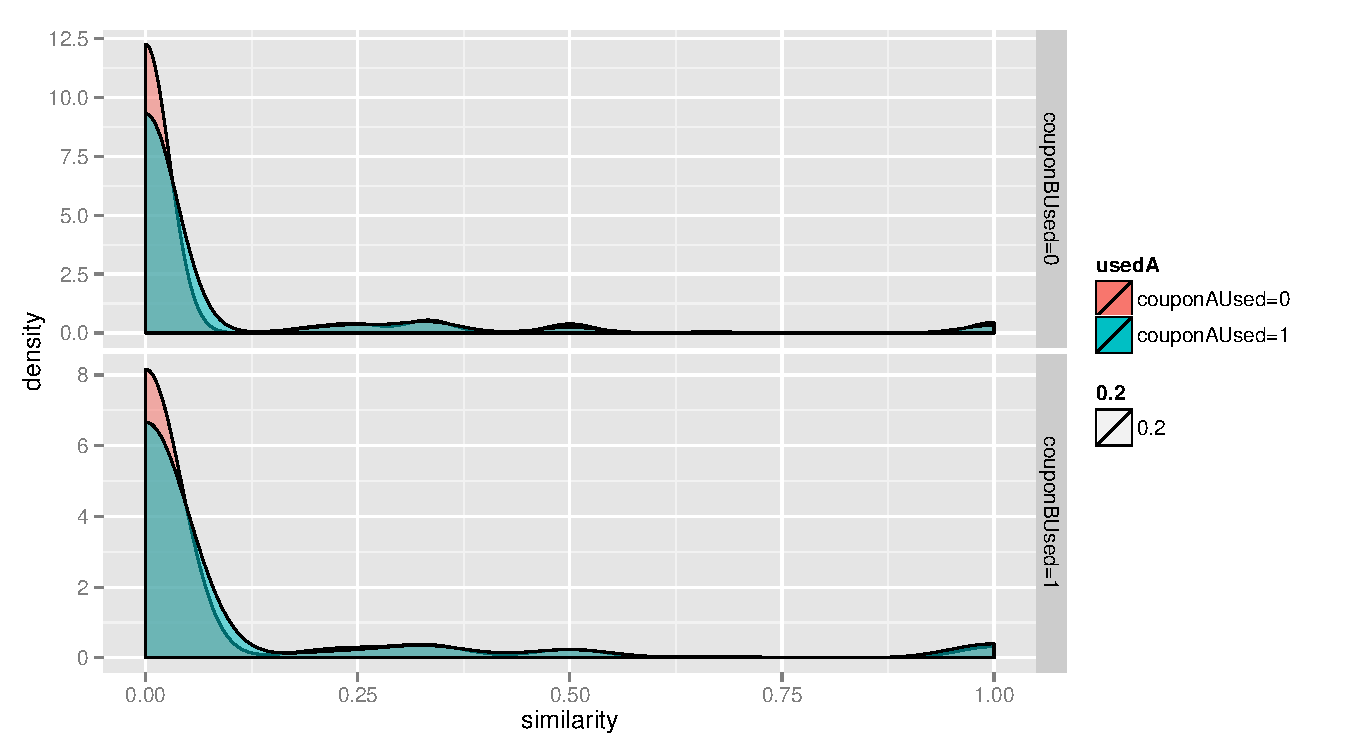
\includegraphics[width=.9\linewidth,height=.5\linewidth]{/Users/user/dmc2015/ian/graphics/fig_unnamed-chunk-8-1} 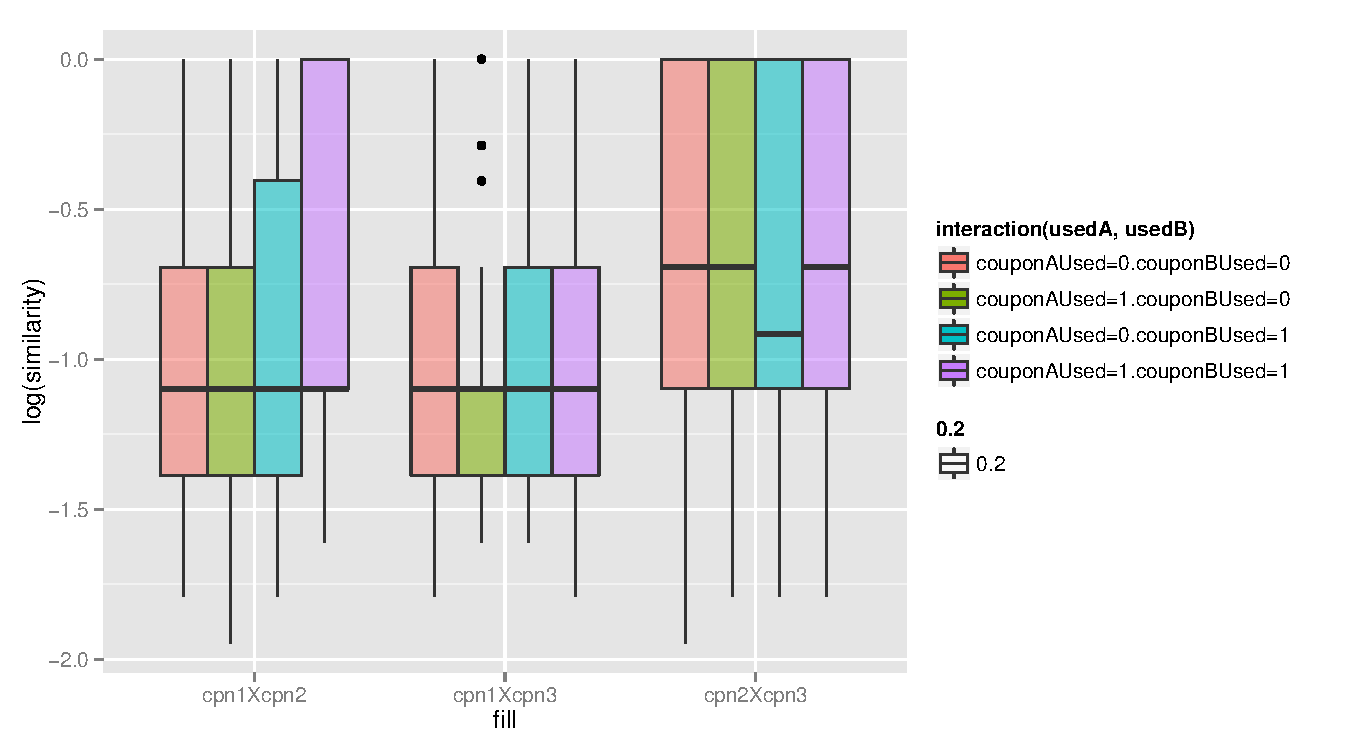
\includegraphics[width=.9\linewidth,height=.5\linewidth]{/Users/user/dmc2015/ian/graphics/fig_unnamed-chunk-8-2} \end{center}

\subsection{tf-idf using ftd and
lnorm}\label{tf-idf-using-ftd-and-lnorm}

\begin{Shaded}
\begin{Highlighting}[]
\CommentTok{# similarity matrix}
\NormalTok{sim_mat =}\StringTok{ }\NormalTok{cos.d1}

\CommentTok{# figures}
\NormalTok{figures =}\StringTok{ }\KeywordTok{simFeatures}\NormalTok{(sim_mat)}

\CommentTok{# print}
\KeywordTok{print}\NormalTok{(figures$p1)}
\KeywordTok{print}\NormalTok{(figures$p2)}
\end{Highlighting}
\end{Shaded}

\begin{verbatim}
## Warning in loop_apply(n, do.ply): Removed 13870 rows containing non-finite
## values (stat_boxplot).
\end{verbatim}

\begin{Shaded}
\begin{Highlighting}[]
\CommentTok{# save}
\KeywordTok{saveRDS}\NormalTok{(sim_mat, }\DataTypeTok{file =} \StringTok{"../features/feature_files/universal/ftd_lnorm_similarity.rds"}\NormalTok{)}
\end{Highlighting}
\end{Shaded}

\begin{center}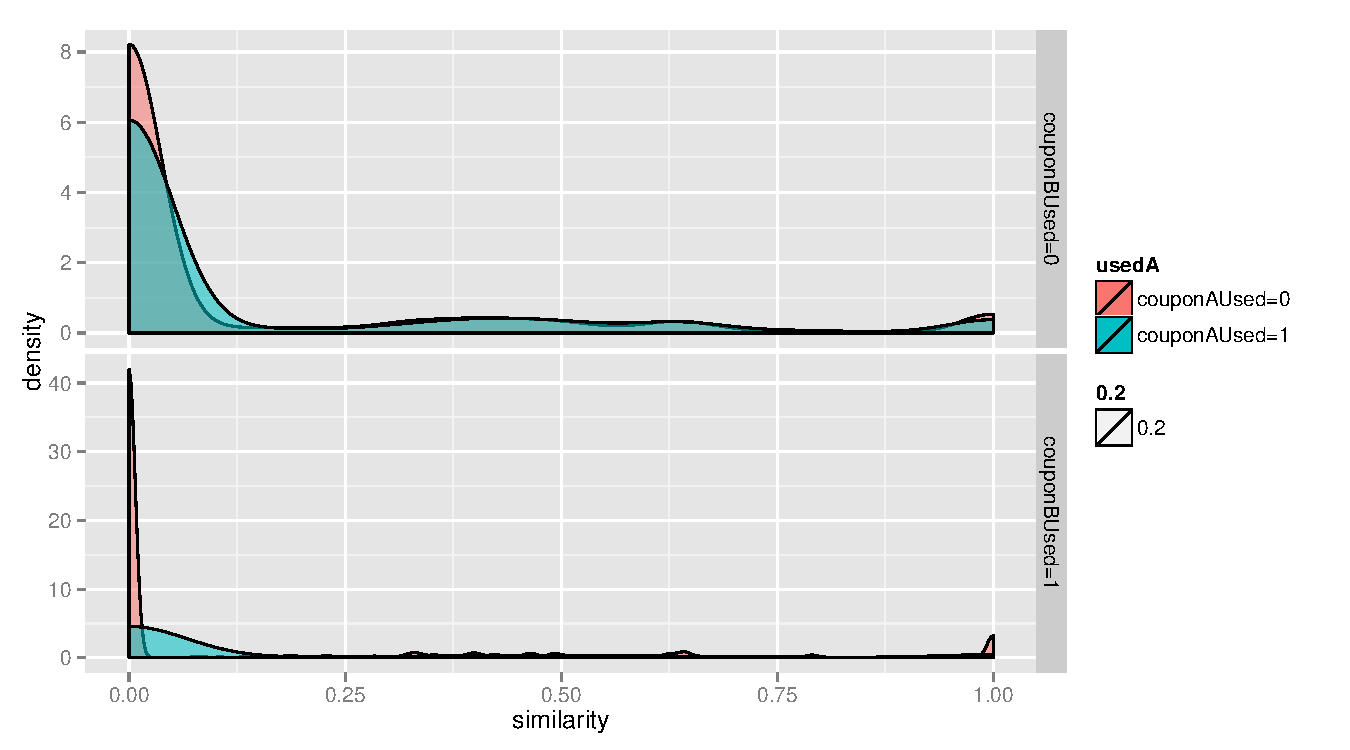
\includegraphics[width=.9\linewidth,height=.5\linewidth]{/Users/user/dmc2015/ian/graphics/fig_unnamed-chunk-9-1} 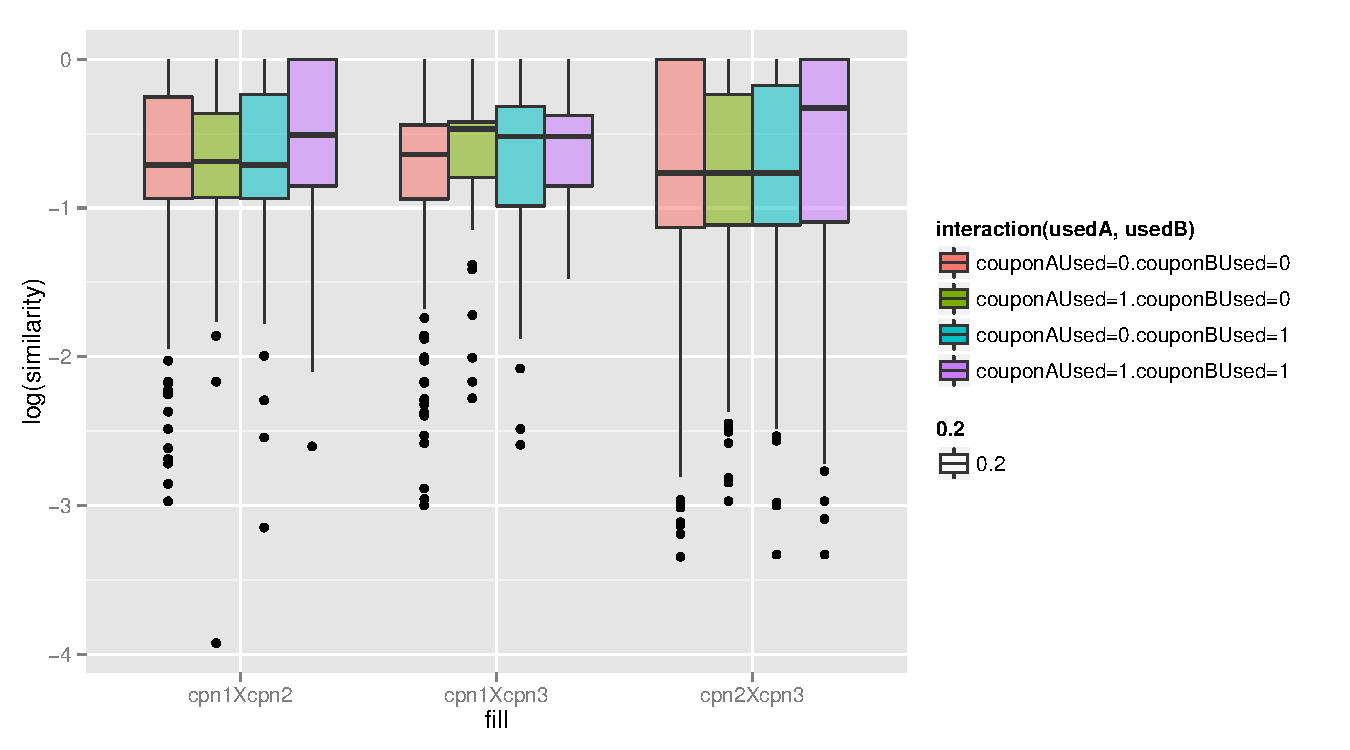
\includegraphics[width=.9\linewidth,height=.5\linewidth]{/Users/user/dmc2015/ian/graphics/fig_unnamed-chunk-9-2} \end{center}

\subsection{tf-idf using ftd and ivf}\label{tf-idf-using-ftd-and-ivf}

\begin{Shaded}
\begin{Highlighting}[]
\CommentTok{# similarity matrix}
\NormalTok{sim_mat =}\StringTok{ }\NormalTok{cos.d2}

\CommentTok{# figures}
\NormalTok{figures =}\StringTok{ }\KeywordTok{simFeatures}\NormalTok{(sim_mat)}

\CommentTok{# print}
\KeywordTok{print}\NormalTok{(figures$p1)}
\KeywordTok{print}\NormalTok{(figures$p2)}
\end{Highlighting}
\end{Shaded}

\begin{verbatim}
## Warning in loop_apply(n, do.ply): Removed 13870 rows containing non-finite
## values (stat_boxplot).
\end{verbatim}

\begin{Shaded}
\begin{Highlighting}[]
\CommentTok{# save}
\KeywordTok{saveRDS}\NormalTok{(sim_mat, }\DataTypeTok{file =} \StringTok{"../features/feature_files/universal/ftd_ivf_similarity.rds"}\NormalTok{)}
\end{Highlighting}
\end{Shaded}

\begin{center}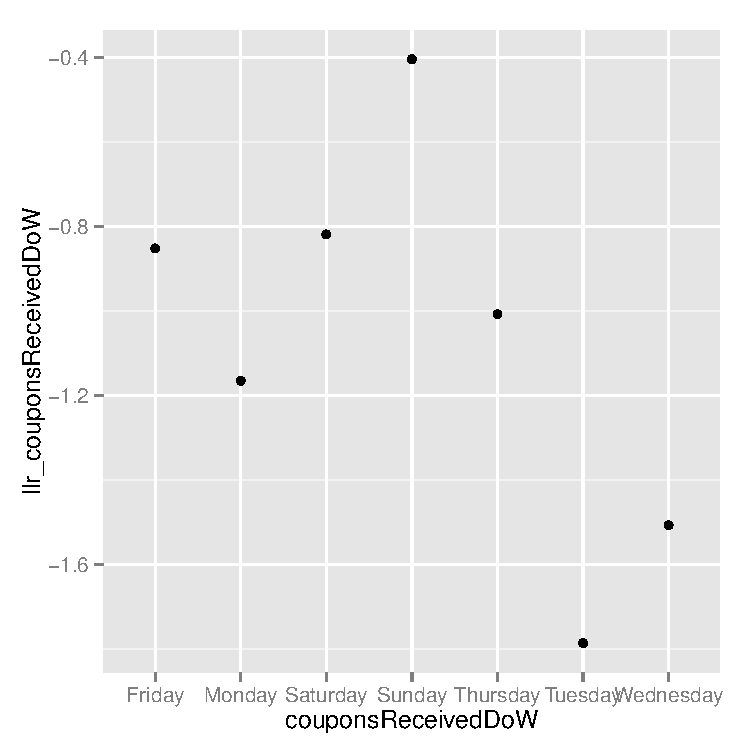
\includegraphics[width=.9\linewidth,height=.5\linewidth]{/Users/user/dmc2015/ian/graphics/fig_unnamed-chunk-10-1} 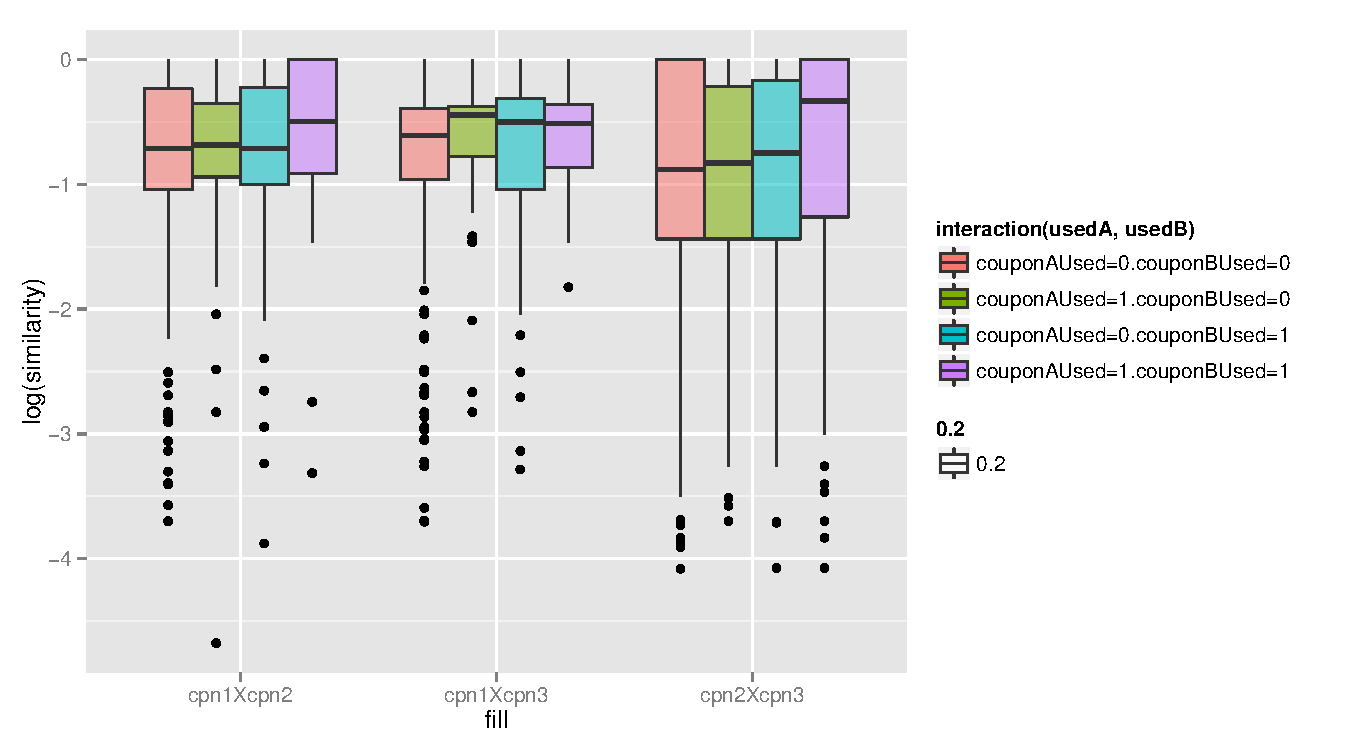
\includegraphics[width=.9\linewidth,height=.5\linewidth]{/Users/user/dmc2015/ian/graphics/fig_unnamed-chunk-10-2} \end{center}

\subsection{tf-idf using ftd and
invmax}\label{tf-idf-using-ftd-and-invmax}

\begin{Shaded}
\begin{Highlighting}[]
\CommentTok{# similarity matrix}
\NormalTok{sim_mat =}\StringTok{ }\NormalTok{cos.d3}

\CommentTok{# figures}
\NormalTok{figures =}\StringTok{ }\KeywordTok{simFeatures}\NormalTok{(sim_mat)}

\CommentTok{# print}
\KeywordTok{print}\NormalTok{(figures$p1)}
\KeywordTok{print}\NormalTok{(figures$p2)}
\end{Highlighting}
\end{Shaded}

\begin{verbatim}
## Warning in loop_apply(n, do.ply): Removed 13870 rows containing non-finite
## values (stat_boxplot).
\end{verbatim}

\begin{Shaded}
\begin{Highlighting}[]
\CommentTok{# save}
\KeywordTok{saveRDS}\NormalTok{(sim_mat, }\DataTypeTok{file =} \StringTok{"../features/feature_files/universal/ftd_invmax_similarity.rds"}\NormalTok{)}
\end{Highlighting}
\end{Shaded}

\begin{center}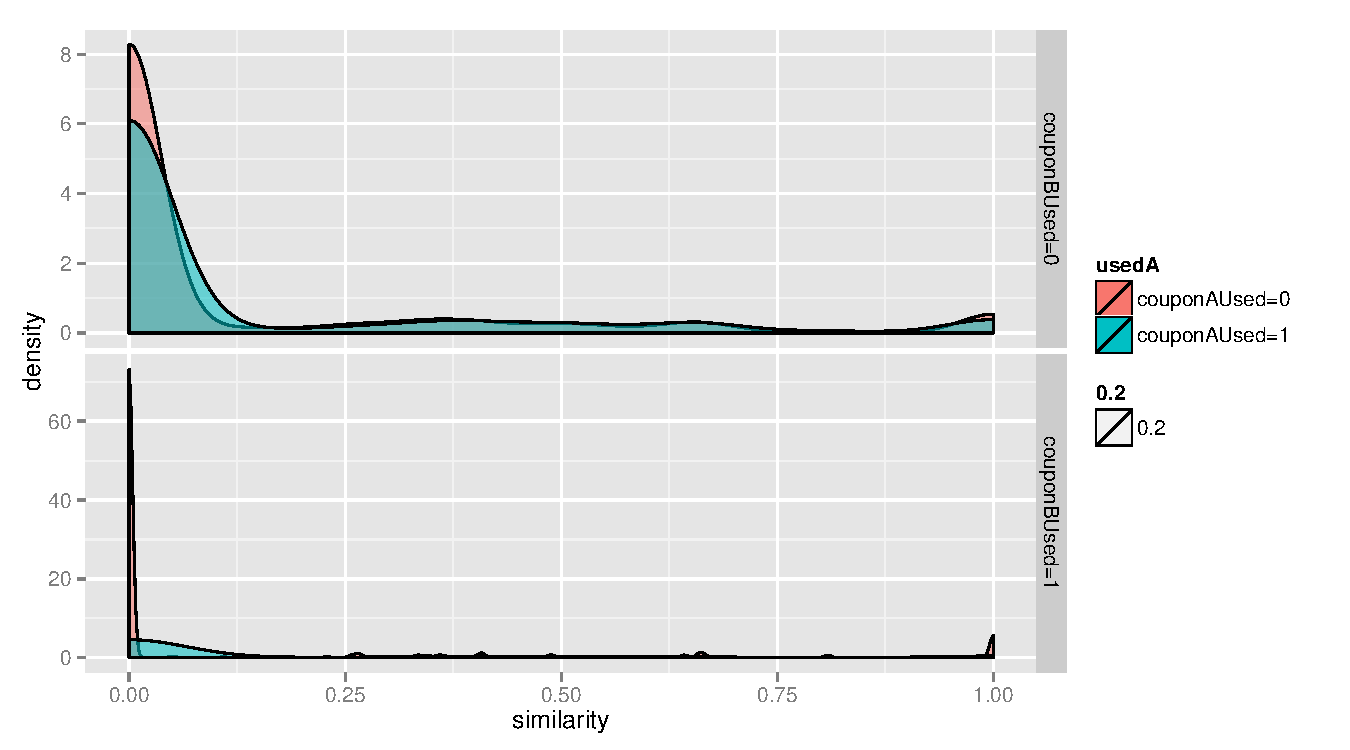
\includegraphics[width=.9\linewidth,height=.5\linewidth]{/Users/user/dmc2015/ian/graphics/fig_unnamed-chunk-11-1} 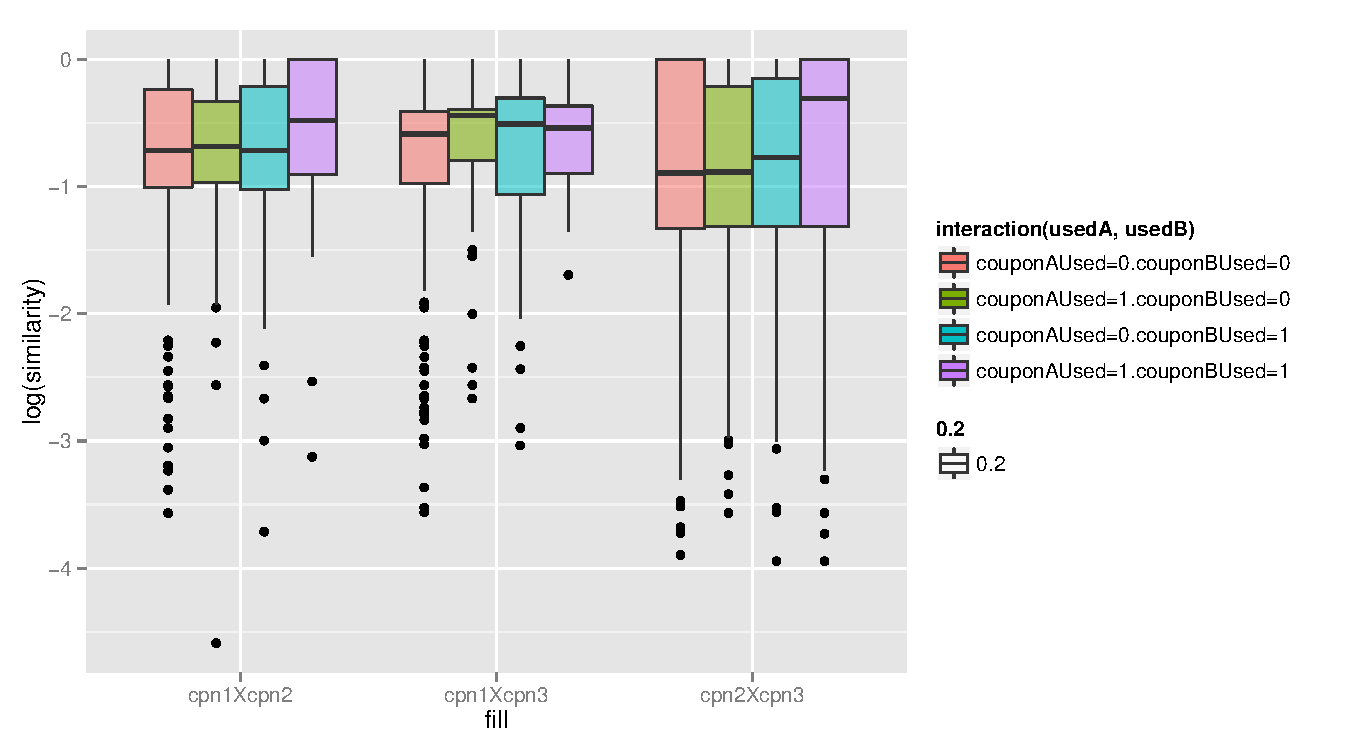
\includegraphics[width=.9\linewidth,height=.5\linewidth]{/Users/user/dmc2015/ian/graphics/fig_unnamed-chunk-11-2} \end{center}

\subsection{tf-idf using ftd and pif}\label{tf-idf-using-ftd-and-pif}

\begin{Shaded}
\begin{Highlighting}[]
\CommentTok{# similarity matrix}
\NormalTok{sim_mat =}\StringTok{ }\NormalTok{cos.d4}

\CommentTok{# figures}
\NormalTok{figures =}\StringTok{ }\KeywordTok{simFeatures}\NormalTok{(sim_mat)}

\CommentTok{# print}
\KeywordTok{print}\NormalTok{(figures$p1)}
\KeywordTok{print}\NormalTok{(figures$p2)}
\end{Highlighting}
\end{Shaded}

\begin{verbatim}
## Warning in loop_apply(n, do.ply): Removed 13870 rows containing non-finite
## values (stat_boxplot).
\end{verbatim}

\begin{Shaded}
\begin{Highlighting}[]
\CommentTok{# save}
\KeywordTok{saveRDS}\NormalTok{(sim_mat, }\DataTypeTok{file =} \StringTok{"../features/feature_files/universal/ftd_pif_similarity.rds"}\NormalTok{)}
\end{Highlighting}
\end{Shaded}

\begin{center}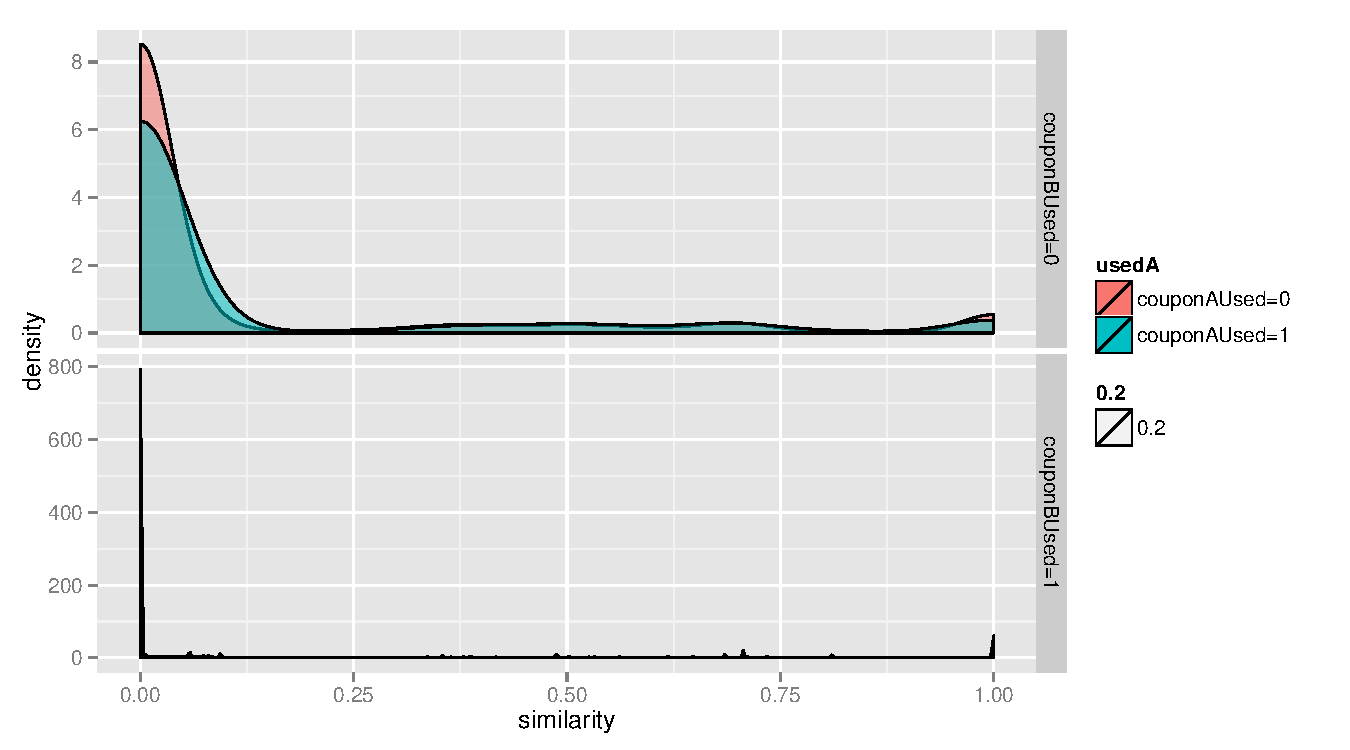
\includegraphics[width=.9\linewidth,height=.5\linewidth]{/Users/user/dmc2015/ian/graphics/fig_unnamed-chunk-12-1} 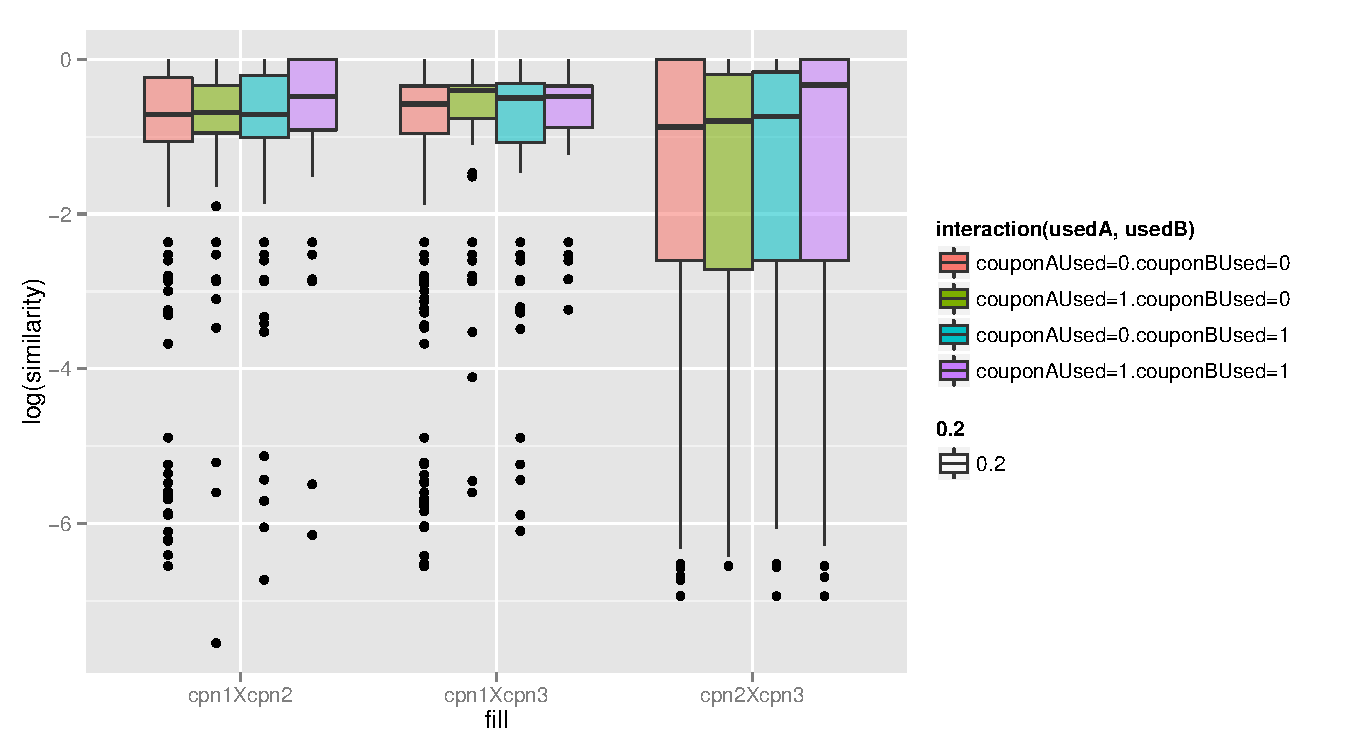
\includegraphics[width=.9\linewidth,height=.5\linewidth]{/Users/user/dmc2015/ian/graphics/fig_unnamed-chunk-12-2} \end{center}

\subsection{tf-idf using lnorm and
lnorm}\label{tf-idf-using-lnorm-and-lnorm}

\begin{Shaded}
\begin{Highlighting}[]
\CommentTok{# similarity matrix}
\NormalTok{sim_mat =}\StringTok{ }\NormalTok{cos.d5}

\CommentTok{# figures}
\NormalTok{figures =}\StringTok{ }\KeywordTok{simFeatures}\NormalTok{(sim_mat)}

\CommentTok{# print}
\KeywordTok{print}\NormalTok{(figures$p1)}
\KeywordTok{print}\NormalTok{(figures$p2)}
\end{Highlighting}
\end{Shaded}

\begin{verbatim}
## Warning in loop_apply(n, do.ply): Removed 13870 rows containing non-finite
## values (stat_boxplot).
\end{verbatim}

\begin{Shaded}
\begin{Highlighting}[]
\CommentTok{# save}
\KeywordTok{saveRDS}\NormalTok{(sim_mat, }\DataTypeTok{file =} \StringTok{"../features/feature_files/universal/lnorm_lnorm_similarity.rds"}\NormalTok{)}
\end{Highlighting}
\end{Shaded}

\begin{center}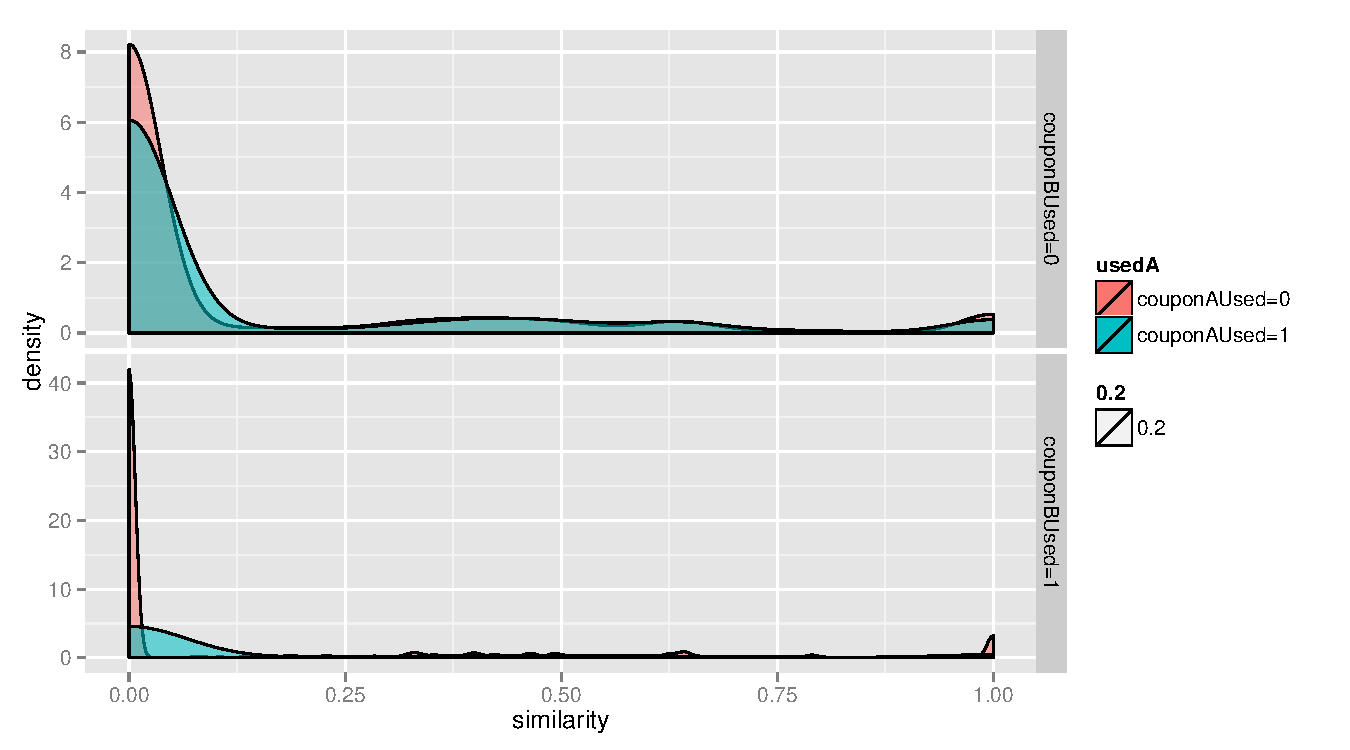
\includegraphics[width=.9\linewidth,height=.5\linewidth]{/Users/user/dmc2015/ian/graphics/fig_unnamed-chunk-13-1} 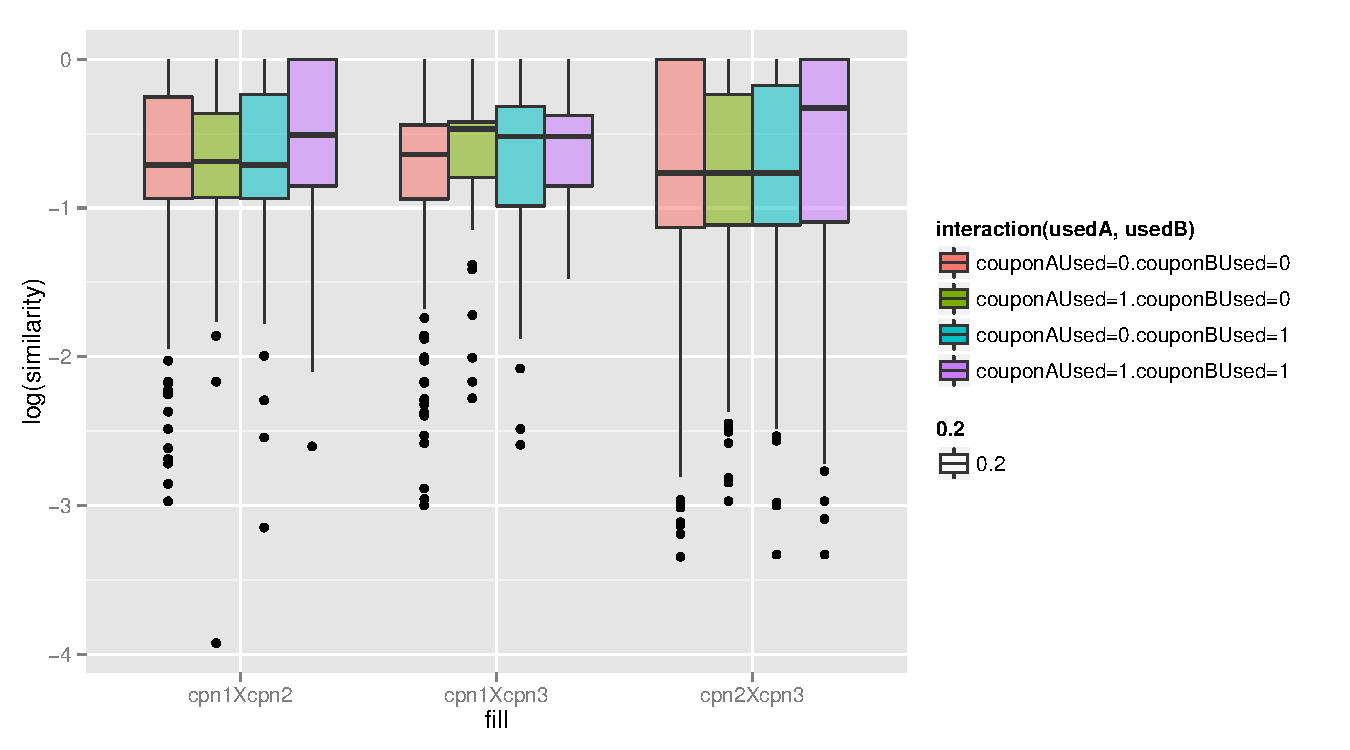
\includegraphics[width=.9\linewidth,height=.5\linewidth]{/Users/user/dmc2015/ian/graphics/fig_unnamed-chunk-13-2} \end{center}

\subsection{tf-idf using lnorm and
ivf}\label{tf-idf-using-lnorm-and-ivf}

\begin{Shaded}
\begin{Highlighting}[]
\CommentTok{# similarity matrix}
\NormalTok{sim_mat =}\StringTok{ }\NormalTok{cos.d6}

\CommentTok{# figures}
\NormalTok{figures =}\StringTok{ }\KeywordTok{simFeatures}\NormalTok{(sim_mat)}

\CommentTok{# print}
\KeywordTok{print}\NormalTok{(figures$p1)}
\KeywordTok{print}\NormalTok{(figures$p2)}
\end{Highlighting}
\end{Shaded}

\begin{verbatim}
## Warning in loop_apply(n, do.ply): Removed 13870 rows containing non-finite
## values (stat_boxplot).
\end{verbatim}

\begin{Shaded}
\begin{Highlighting}[]
\CommentTok{# save}
\KeywordTok{saveRDS}\NormalTok{(sim_mat, }\DataTypeTok{file =} \StringTok{"../features/feature_files/universal/lnorm_ivf_similarity.rds"}\NormalTok{)}
\end{Highlighting}
\end{Shaded}

\begin{center}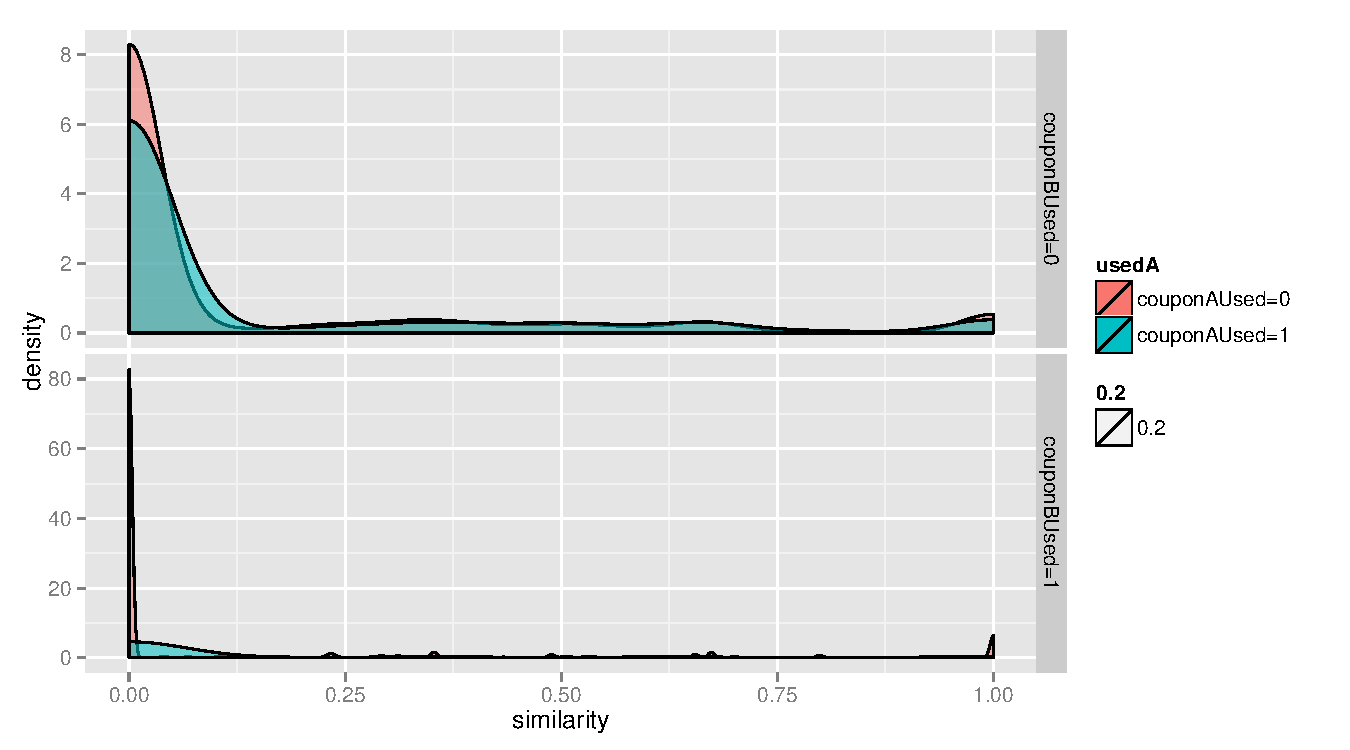
\includegraphics[width=.9\linewidth,height=.5\linewidth]{/Users/user/dmc2015/ian/graphics/fig_unnamed-chunk-14-1} 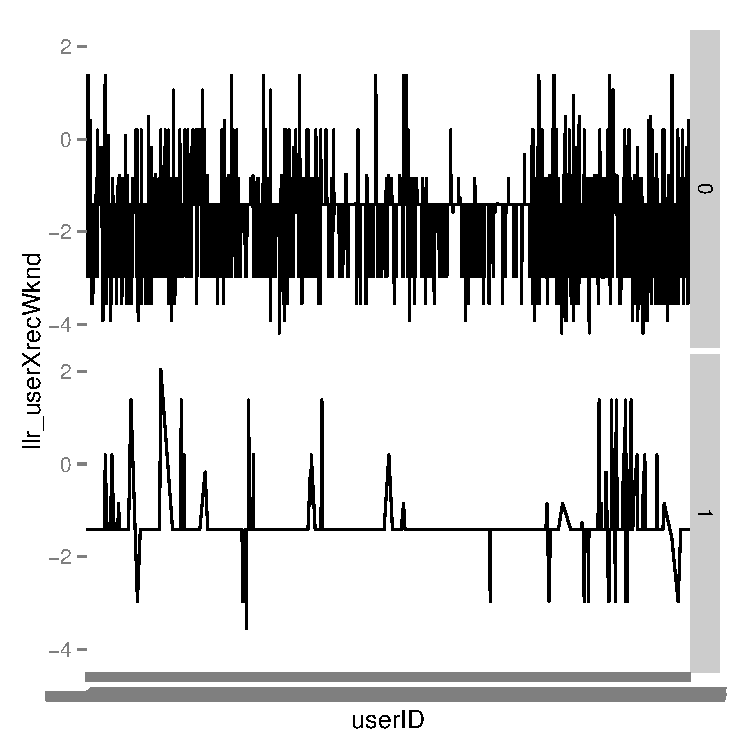
\includegraphics[width=.9\linewidth,height=.5\linewidth]{/Users/user/dmc2015/ian/graphics/fig_unnamed-chunk-14-2} \end{center}

\subsection{tf-idf using lnorm and
invmax}\label{tf-idf-using-lnorm-and-invmax}

\begin{Shaded}
\begin{Highlighting}[]
\CommentTok{# similarity matrix}
\NormalTok{sim_mat =}\StringTok{ }\NormalTok{cos.d7}

\CommentTok{# figures}
\NormalTok{figures =}\StringTok{ }\KeywordTok{simFeatures}\NormalTok{(sim_mat)}

\CommentTok{# print}
\KeywordTok{print}\NormalTok{(figures$p1)}
\KeywordTok{print}\NormalTok{(figures$p2)}
\end{Highlighting}
\end{Shaded}

\begin{verbatim}
## Warning in loop_apply(n, do.ply): Removed 13870 rows containing non-finite
## values (stat_boxplot).
\end{verbatim}

\begin{Shaded}
\begin{Highlighting}[]
\CommentTok{# save}
\KeywordTok{saveRDS}\NormalTok{(sim_mat, }\DataTypeTok{file =} \StringTok{"../features/feature_files/universal/lnorm_invmax_similarity.rds"}\NormalTok{)}
\end{Highlighting}
\end{Shaded}

\begin{center}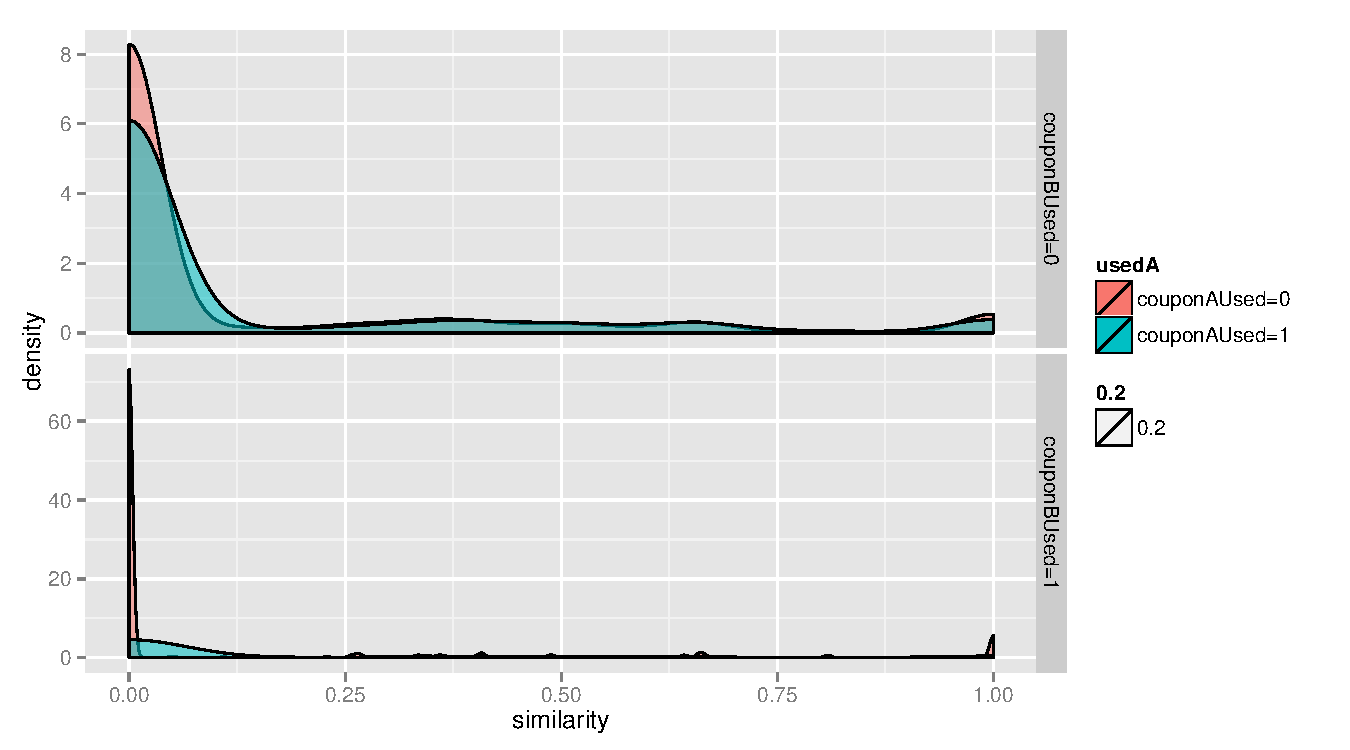
\includegraphics[width=.9\linewidth,height=.5\linewidth]{/Users/user/dmc2015/ian/graphics/fig_unnamed-chunk-15-1} 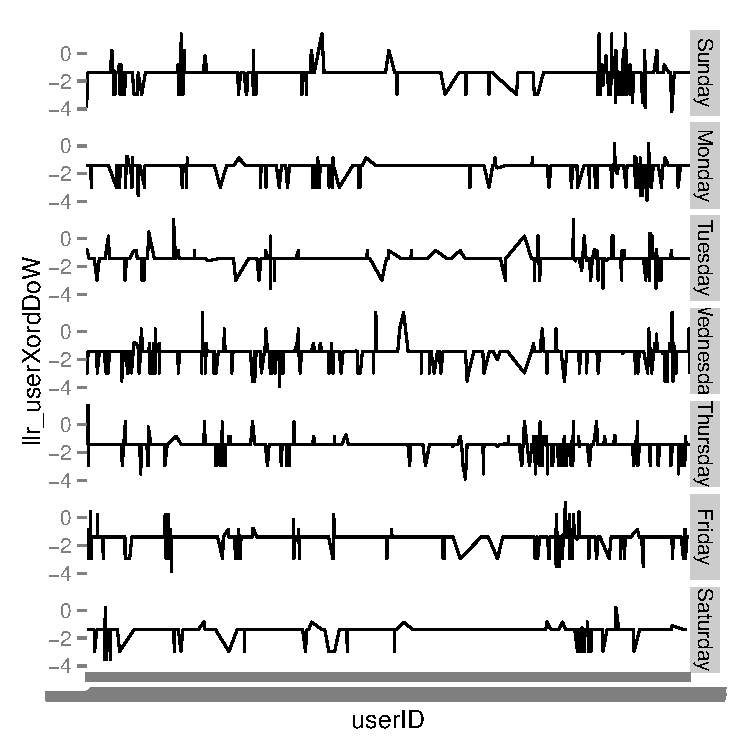
\includegraphics[width=.9\linewidth,height=.5\linewidth]{/Users/user/dmc2015/ian/graphics/fig_unnamed-chunk-15-2} \end{center}

\subsection{tf-idf using lnorm and
pif}\label{tf-idf-using-lnorm-and-pif}

\begin{Shaded}
\begin{Highlighting}[]
\CommentTok{# similarity matrix}
\NormalTok{sim_mat =}\StringTok{ }\NormalTok{cos.d8}

\CommentTok{# figures}
\NormalTok{figures =}\StringTok{ }\KeywordTok{simFeatures}\NormalTok{(sim_mat)}

\CommentTok{# print}
\KeywordTok{print}\NormalTok{(figures$p1)}
\KeywordTok{print}\NormalTok{(figures$p2)}
\end{Highlighting}
\end{Shaded}

\begin{verbatim}
## Warning in loop_apply(n, do.ply): Removed 13870 rows containing non-finite
## values (stat_boxplot).
\end{verbatim}

\begin{Shaded}
\begin{Highlighting}[]
\CommentTok{# save}
\KeywordTok{saveRDS}\NormalTok{(sim_mat, }\DataTypeTok{file =} \StringTok{"../features/feature_files/universal/lnorm_pif_similarity.rds"}\NormalTok{)}
\end{Highlighting}
\end{Shaded}

\begin{center}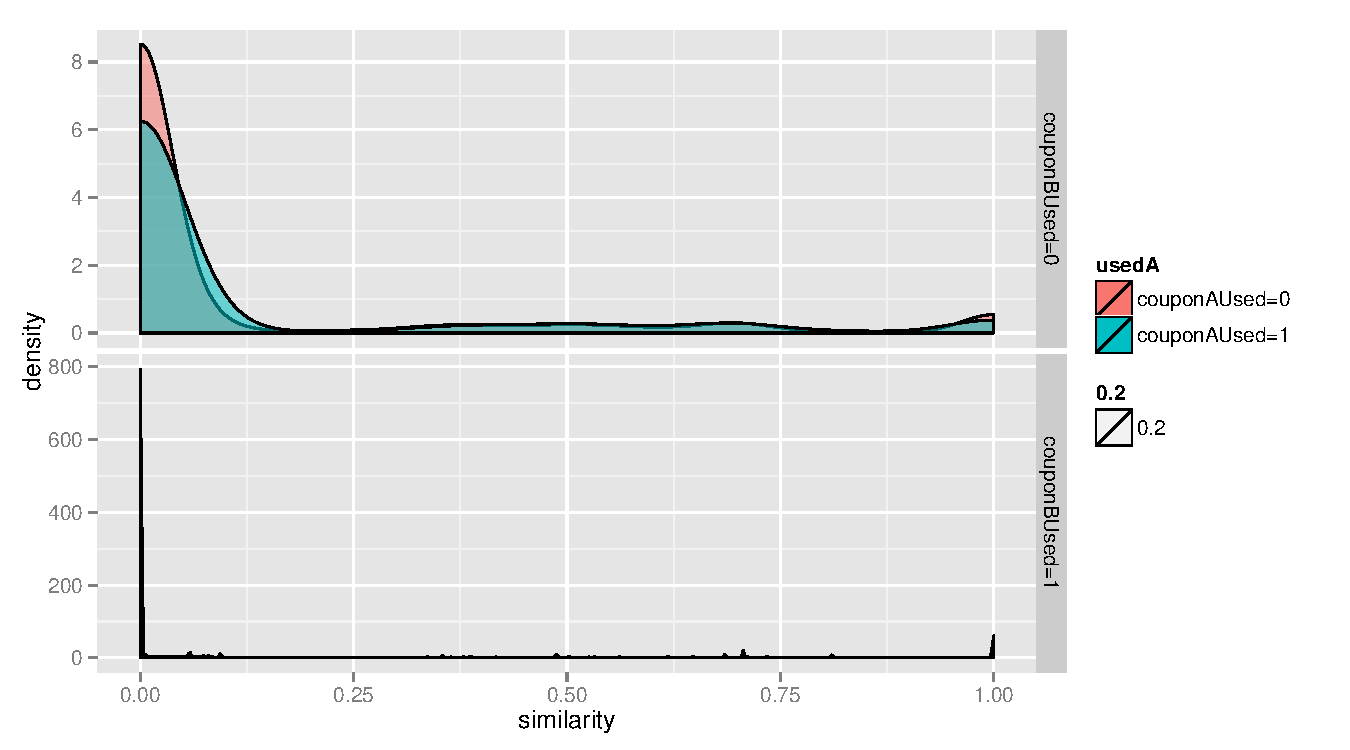
\includegraphics[width=.9\linewidth,height=.5\linewidth]{/Users/user/dmc2015/ian/graphics/fig_unnamed-chunk-16-1} 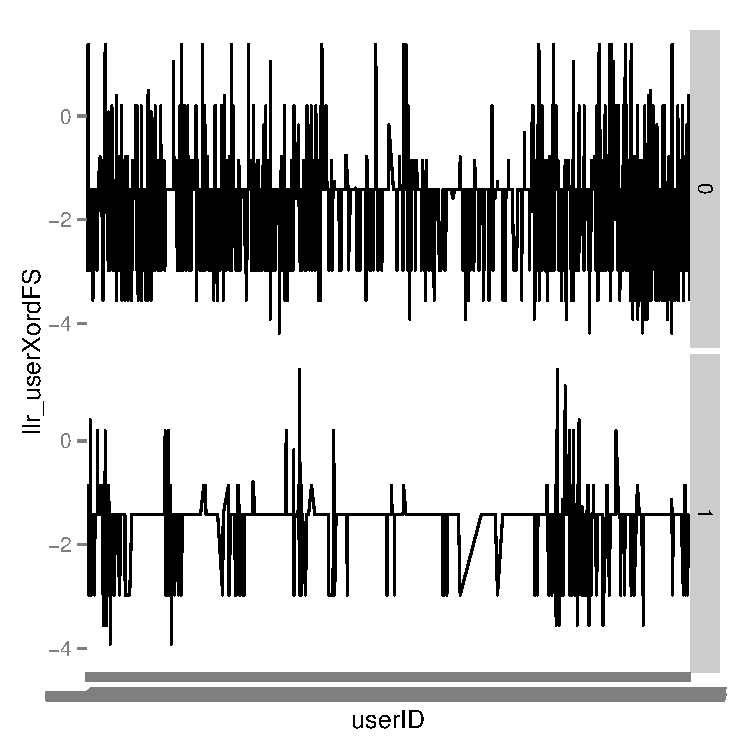
\includegraphics[width=.9\linewidth,height=.5\linewidth]{/Users/user/dmc2015/ian/graphics/fig_unnamed-chunk-16-2} \end{center}

\end{document}
